\documentclass[12pt,a4paper]{ctexart}
\usepackage[margin=2.2cm]{geometry}
\usepackage{booktabs}
\usepackage{array}
\usepackage{graphicx}
\usepackage{float}
\usepackage{caption}
\usepackage{subcaption}
\usepackage{hyperref}
\usepackage{siunitx}
\usepackage{xcolor}

\title{CentralLNM 任务性能排查与对照实验报告（重构版）}
\author{PTMC\_LNM 项目分析记录}
\date{\today}

\begin{document}
\maketitle

\begin{abstract}
本文系统汇报 CentralLNM 任务的多阶段对照实验：首先完成数据泄漏与日志可信度排查，并通过 A/B/C 单任务实验确认泛化落差客观存在；随后在患者级 5-fold 上开展深度学习三路对照（clinical-only、image-only、clinical+DeepRadScore）与可解释性分析；进一步补充传统机器学习三路对照（clinical-only、radiomics-only、clinical+radiomics）及多模型比较（LogReg、RandomForest、SVM、AdaBoost、ExtraTrees、Stacking、SoftVoting）。报告统一给出 5-fold 明细、均值$\pm$标准差、ROC/箱线图和复现清单。综合结果表明：临床特征是当前最稳健信号来源，影像分支（无论深度特征还是传统影像组学）可提供辅助信息但尚未形成稳定增益。
\end{abstract}

\tableofcontents
\newpage

\section{问题背景与目标}

\subsection{初始现象}
\begin{itemize}
  \item 训练集 AUC 很快升高并接近 1；
  \item 验证/测试集 AUC 长期在 0.55$\sim$0.65 波动；
  \item 存在明显泛化落差（Train $\gg$ Val/Test）。
\end{itemize}

\subsection{本报告目标}
\begin{enumerate}
  \item 排除数据泄漏与划分问题；
  \item 修正训练日志可信度并复核泛化差距；
  \item 从临床、深度学习、传统影像组学三条路线做患者级 5-fold 对照；
  \item 输出可复现实验文档与下一轮路线图。
\end{enumerate}

\section{实验 1：数据与日志可信度排查（A/B/C）}

\subsection{实验目的}
验证“训练好、验证差”是否由数据泄漏或日志统计偏差导致，并用 A/B/C 对照确认基础泛化边界。

\subsection{设置}
\begin{itemize}
  \item 数据检查：train/val/test 的样本级与患者级交集检查、标签分布检查；
  \item 日志修正：新增 \texttt{train\_eval\_loader}（不重采样、无增强）用于真实 Train 评估；
  \item A/B/C：
  \begin{itemize}
    \item A：强正则 + ResNet18 + BCE；
    \item B：去临床，仅三模态图像；
    \item C：仅 B 模态 + 临床。
  \end{itemize}
\end{itemize}

\subsection{定量表格}
\begin{table}[H]
\centering
\caption{数据泄漏与标签分布检查结果}
\begin{tabular}{lcc}
\toprule
检查项 & 结果 & 结论 \\
\midrule
同名样本 train$\cap$val / train$\cap$test / val$\cap$test & 全部为 0 & 无样本泄漏 \\
患者 ID train$\cap$val / train$\cap$test / val$\cap$test & 全部为 0 & 无患者泄漏 \\
CentralLNM 阳性率（train/val/test） & 0.534 / 0.532 / 0.478 & 分布接近 \\
\bottomrule
\end{tabular}
\end{table}

\begin{table}[H]
\centering
\caption{A/B/C 对照实验结果（CentralLNM）}
\begin{tabular}{lccc}
\toprule
实验 & Train AUC（eval） & Val AUC & Test AUC \\
\midrule
A（强正则 + ResNet18 + BCE） & 0.9294 & 0.6105 & 0.5306 \\
B（去临床，三模态图像） & 0.9939 & 0.5597 & 0.5569 \\
C（仅 B 模态 + 临床） & 0.9850 & 0.6393 & 0.5099 \\
\bottomrule
\end{tabular}
\end{table}

\subsection{对应图}
\begin{figure}[H]
  \centering
  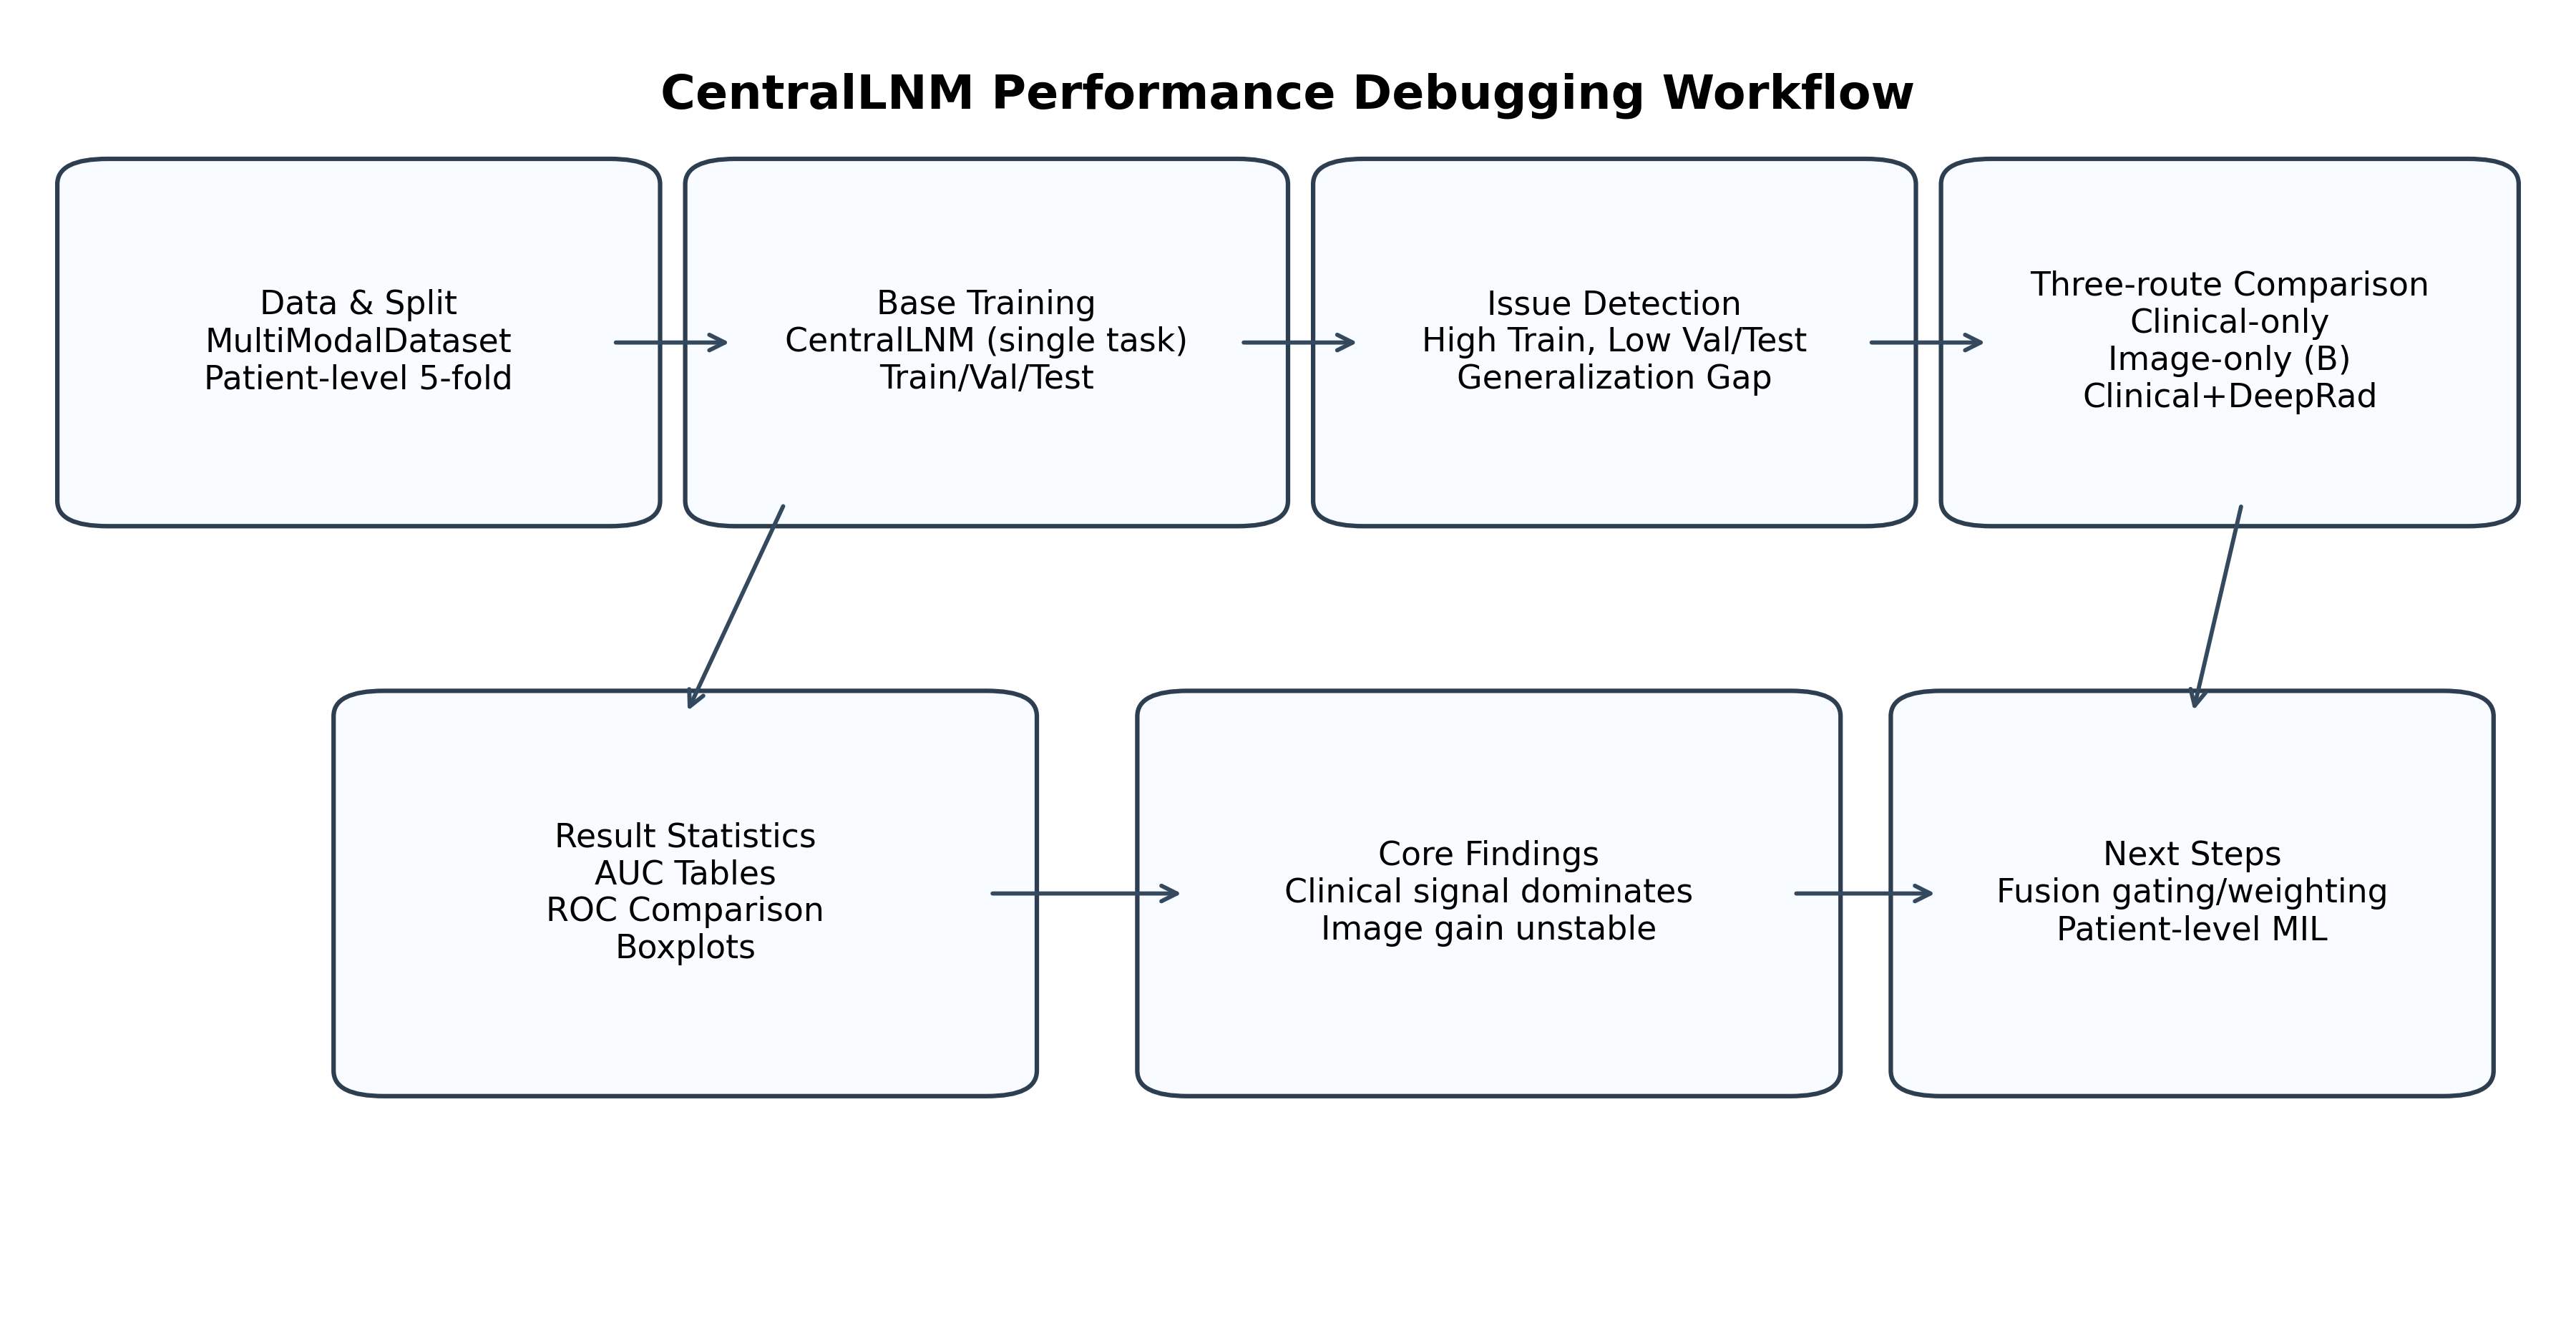
\includegraphics[width=0.90\textwidth]{figures/method_flow_diagram.png}
  \caption{整体排查流程：数据检查、日志修正、患者级验证、三路对照与可解释性分析。}
\end{figure}

\subsection{小结}
\begin{itemize}
  \item 泄漏已排除，Train 高并非由样本重复或患者混入导致；
  \item 日志可信度修正后，Train 仍显著高于 Val/Test，说明泛化问题客观存在；
  \item A/B/C 均未打破“高训练、低外推”的核心模式。
\end{itemize}

\section{实验 2：患者级 5-fold 与 image-only 稳定性}

\subsection{实验目的}
确认泛化问题是否由单次划分偶然性造成，并评估图像分支在患者级聚合下的稳定性。

\subsection{设置}
\begin{itemize}
  \item 患者级 5-fold 交叉验证；
  \item image-only(B) 结果使用患者级概率聚合（max / mean / top3-mean）；
  \item ROC 使用每折 test 集患者级概率绘制叠加曲线。
\end{itemize}

\subsection{定量表格}
\begin{table}[H]
\centering
\caption{患者级 5-fold（CentralLNM）best val AUC}
\begin{tabular}{cc}
\toprule
Fold & Best Val AUC \\
\midrule
0 & 0.6453 \\
1 & 0.6261 \\
2 & 0.5545 \\
3 & 0.5956 \\
4 & 0.5344 \\
\bottomrule
\end{tabular}
\end{table}

\begin{table}[H]
\centering
\caption{Image-only(B) 在患者级聚合下的 test AUC}
\begin{tabular}{cccc}
\toprule
Fold & AUC(max) & AUC(mean) & AUC(top3-mean) \\
\midrule
0 & 0.5734 & 0.5766 & 0.5739 \\
1 & 0.6207 & 0.6293 & 0.6202 \\
2 & 0.5925 & 0.6077 & 0.5968 \\
3 & 0.4790 & 0.5390 & 0.5352 \\
4 & 0.5686 & 0.5741 & 0.5546 \\
\bottomrule
\end{tabular}
\end{table}

\subsection{对应图}
\begin{figure}[H]
  \centering
  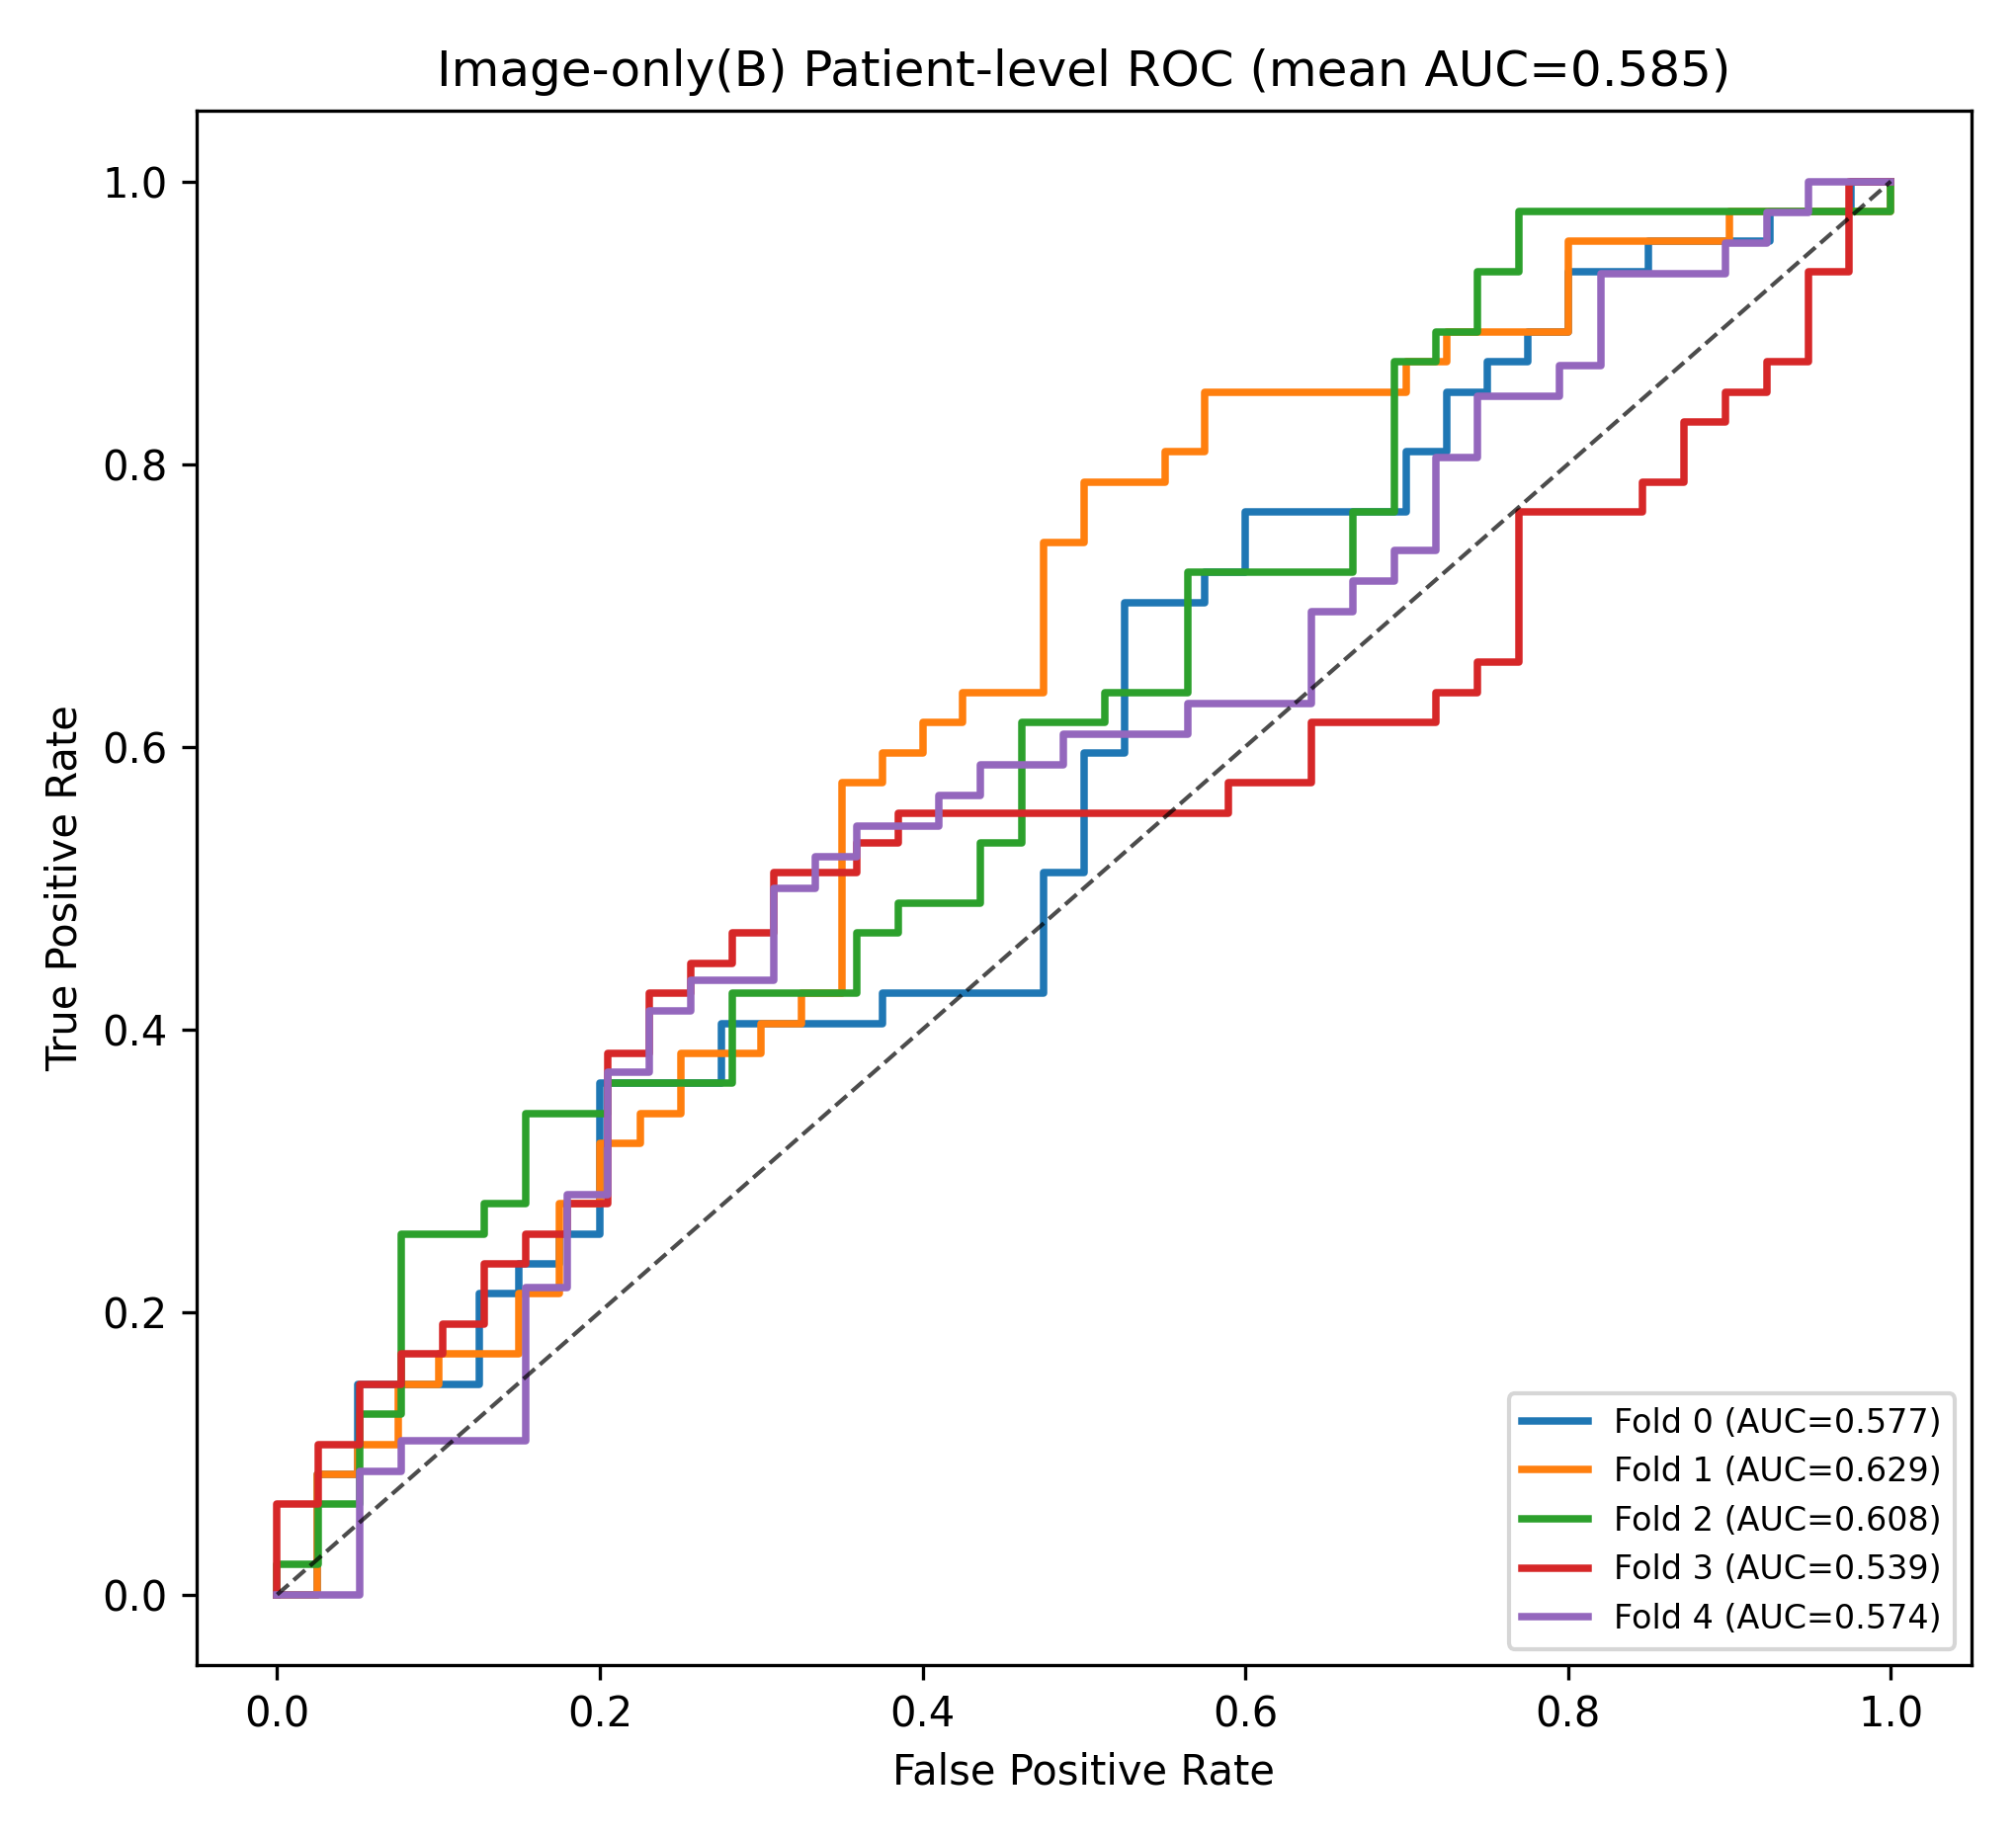
\includegraphics[width=0.74\textwidth]{figures/roc_overlay_imageonly_b.png}
  \caption{Image-only(B) 患者级 ROC 叠加图（5-fold，mean 聚合）。}
\end{figure}

\subsection{小结}
\begin{itemize}
  \item 各折 best val AUC 普遍在 0.53$\sim$0.65，问题不是单次划分偶然；
  \item image-only 的聚合策略（max/mean/top3）未带来稳定提升；
  \item ROC 折间离散明显，图像分支稳定性不足。
\end{itemize}

\section{实验 3：三路总对照（clinical-only / image-only / fusion）}

\subsection{实验目的}
对比不同信息路径的泛化能力，判断图像分支是否提供可复现的增益。

\subsection{设置}
\begin{itemize}
  \item Clinical-only：患者级 LogisticRegression；
  \item Image-only：仅 B 模态深度模型，患者级 mean 聚合；
  \item Fusion：Clinical + DeepRadScore；
  \item 统一在 5-fold test 上比较。
\end{itemize}

\paragraph{DeepRadScore 是什么（通俗解释）}
DeepRadScore 可以理解为“图像分支给每位患者的一个 1 维分数”。
具体做法是：先用 image-only(B) 模型提取每个切片的深度特征（fused），再聚合成患者级向量（mean），然后用 PCA 压缩成 1 个数（只在 train 上拟合），最后把该分数与临床特征拼接后做 LogisticRegression。

\paragraph{消歧说明}
本文中的 DeepRadScore \textbf{不是}传统手工放射组学（handcrafted radiomics）特征，也不是手工勾画后提取的纹理统计量；它是由深度网络自动学习得到的 embedding 经 PCA 压缩后的患者级分数。

\begin{figure}[H]
  \centering
  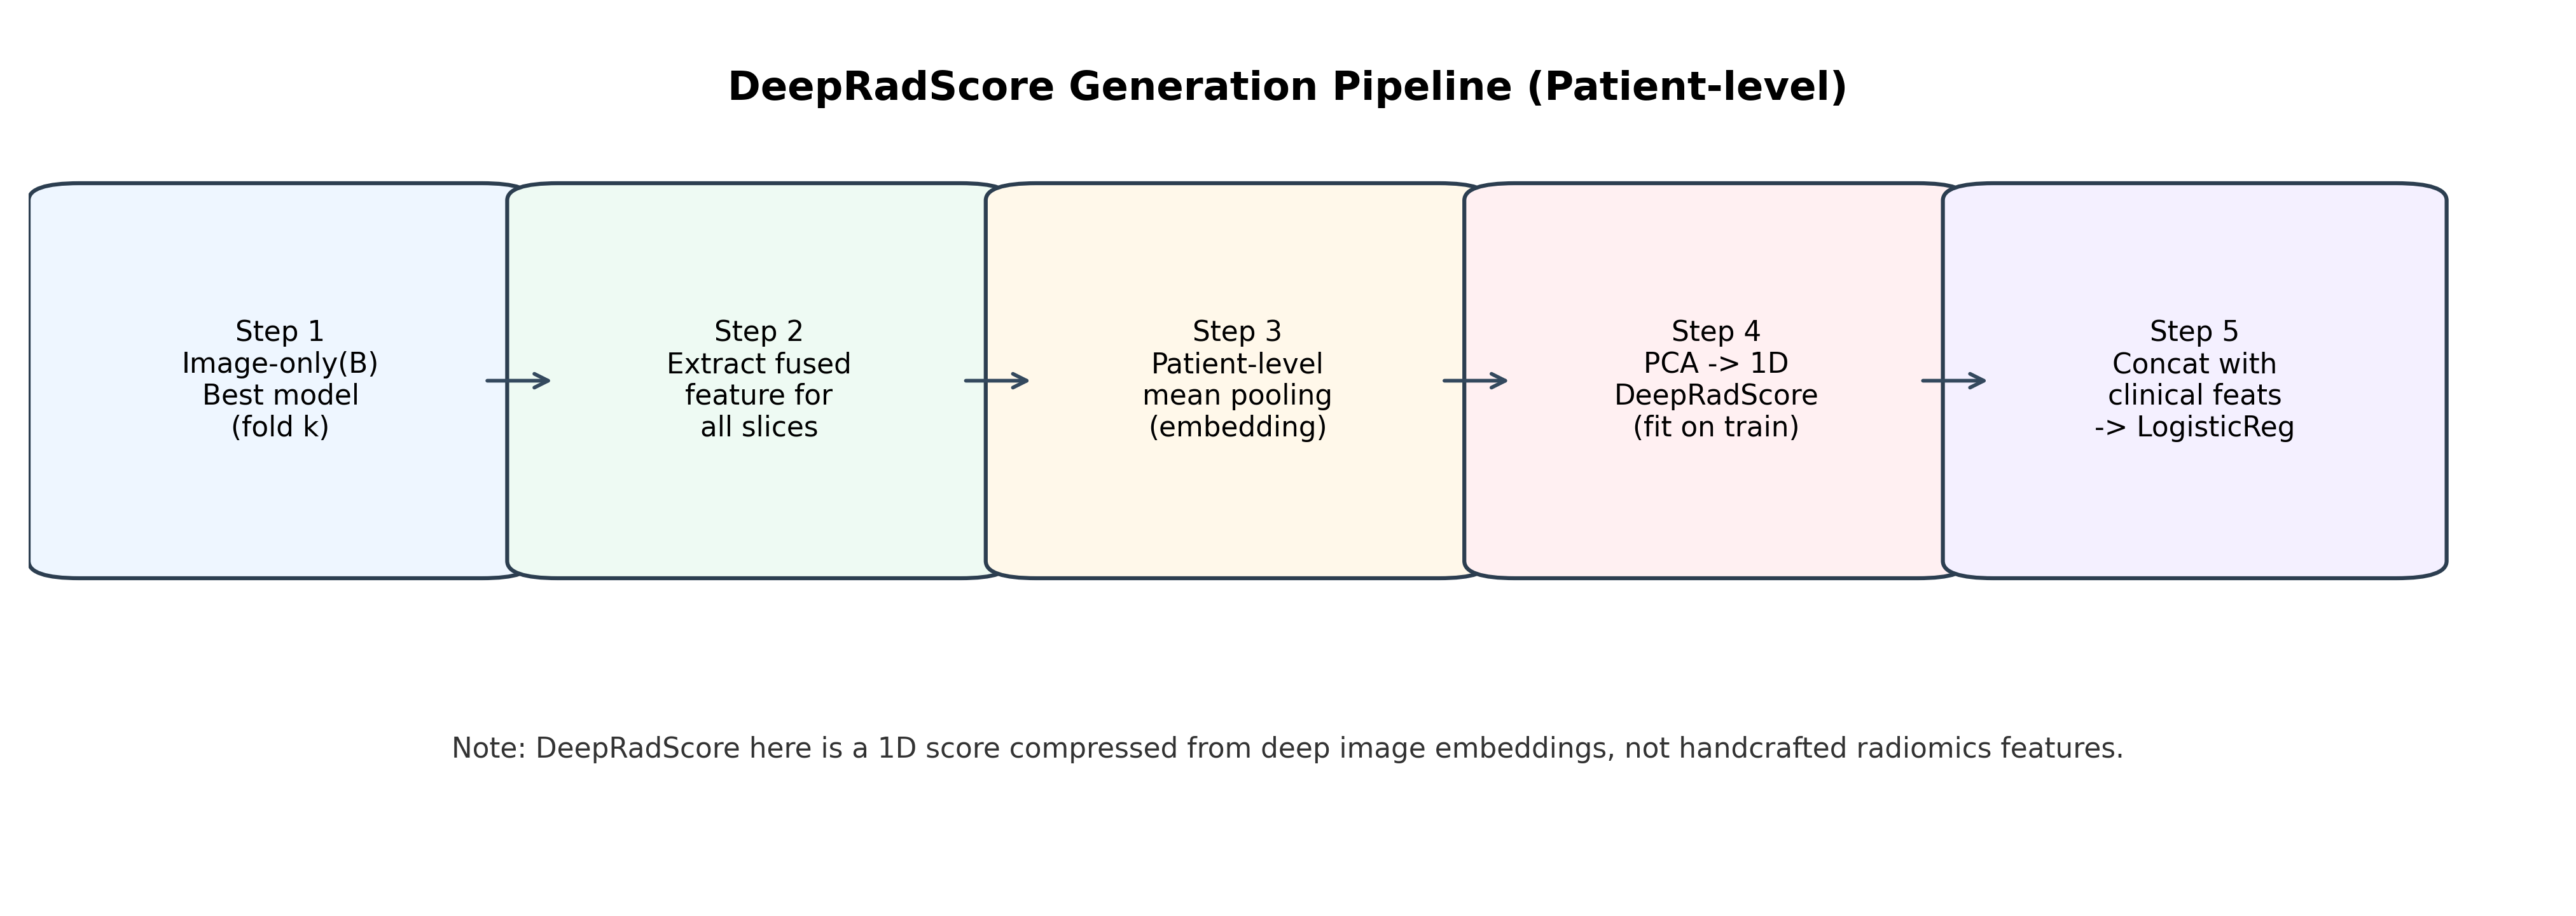
\includegraphics[width=0.95\textwidth]{figures/deepradscore_pipeline.png}
  \caption{DeepRadScore 生成流程图：image-only 特征提取 $\rightarrow$ 患者级聚合 $\rightarrow$ PCA 压缩 $\rightarrow$ 与临床特征拼接建模。}
\end{figure}

\subsection{定量表格}
\begin{table}[H]
\centering
\caption{三路方法 5-fold test AUC 明细}
\begin{tabular}{lccccc}
\toprule
方法 & Fold0 & Fold1 & Fold2 & Fold3 & Fold4 \\
\midrule
Clinical-only（mean+max） & 0.7170 & 0.7239 & 0.6454 & 0.6896 & 0.6856 \\
Image-only(B)（mean） & 0.5766 & 0.6293 & 0.6077 & 0.5390 & 0.5741 \\
Clinical+DeepRadScore & 0.7101 & 0.7229 & 0.6448 & 0.6476 & 0.6918 \\
\bottomrule
\end{tabular}
\end{table}

\begin{table}[H]
\centering
\caption{统计稳定性汇总（5-fold，均值$\pm$标准差）}
\begin{tabular}{lccc}
\toprule
方法 & Mean$\pm$Std & Min & Max \\
\midrule
Clinical-only（mean+max） & 0.6923 $\pm$ 0.0311 & 0.6454 & 0.7239 \\
Image-only(B)（mean） & 0.5853 $\pm$ 0.0346 & 0.5390 & 0.6293 \\
Clinical+DeepRadScore & 0.6834 $\pm$ 0.0358 & 0.6448 & 0.7229 \\
\bottomrule
\end{tabular}
\end{table}

\subsection{统计稳定性说明}
\begin{itemize}
  \item 统一采用 5-fold test AUC 的均值$\pm$标准差作为主比较指标，避免只看单折结果；
  \item Clinical-only 的标准差最低且均值最高，说明其当前阶段最稳健；
  \item Fusion 与 Clinical-only 均值接近但标准差更高，提示融合收益尚不稳定。
\end{itemize}

\subsection{对应图}
\begin{figure}[H]
  \centering
  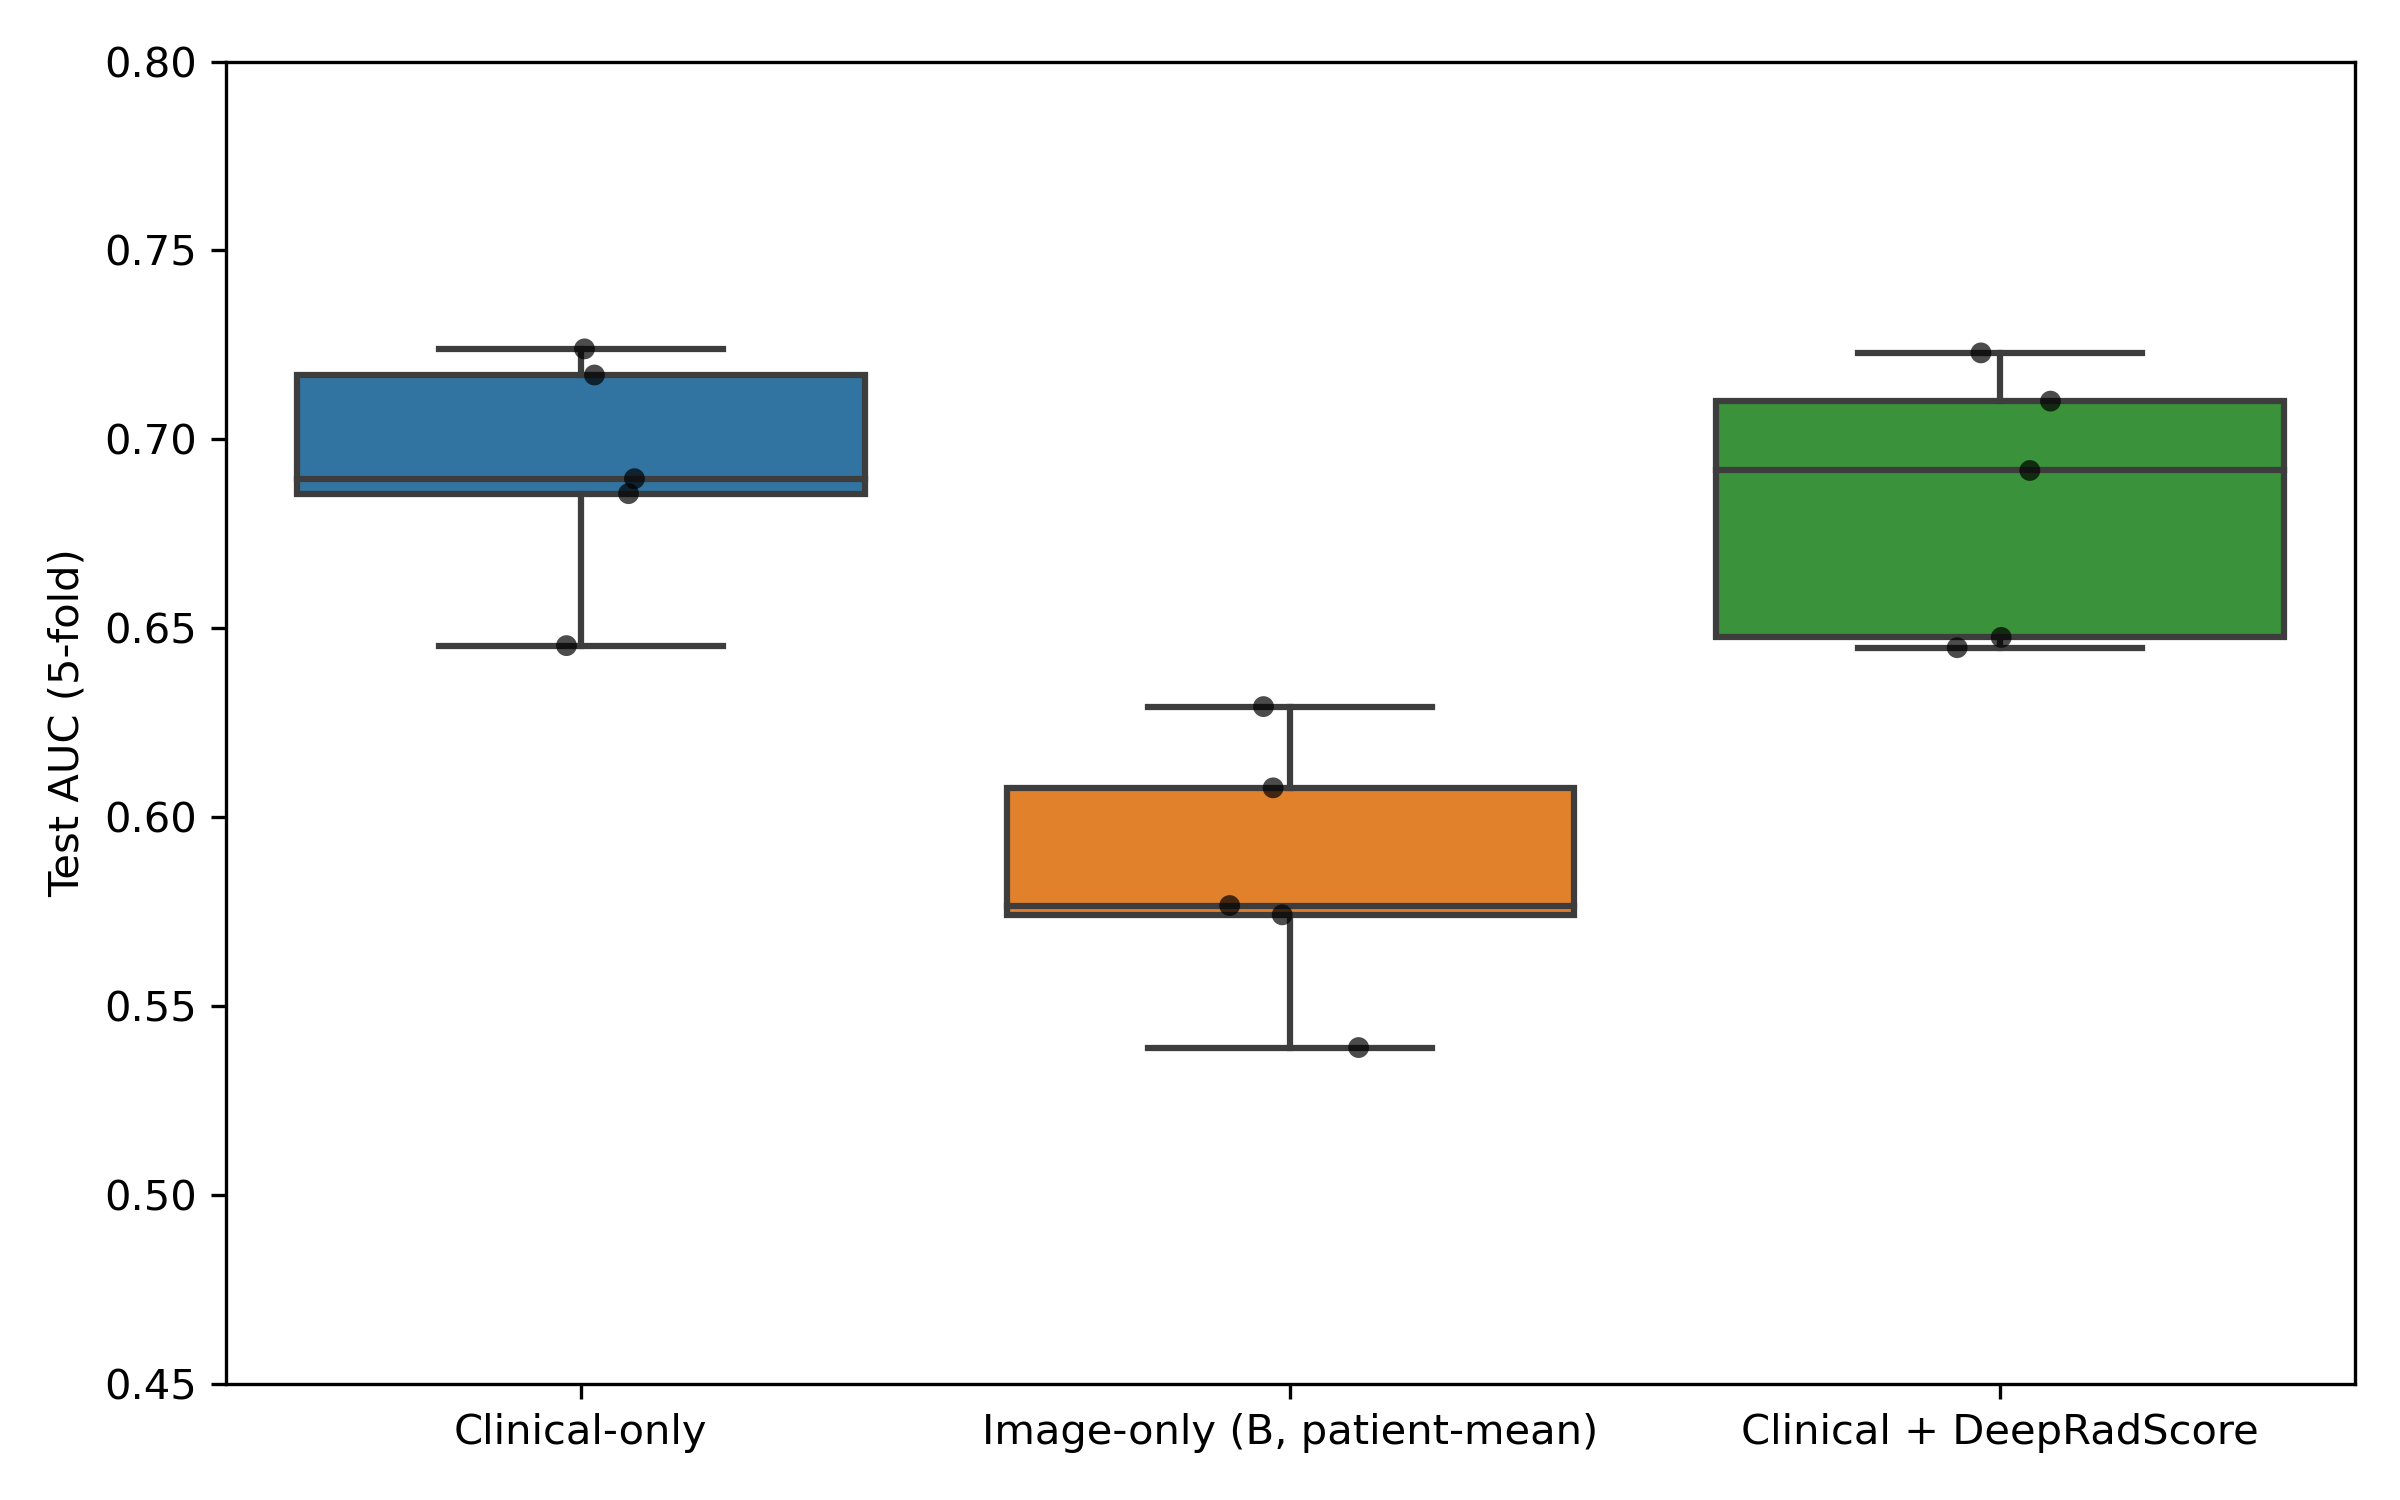
\includegraphics[width=0.82\textwidth]{figures/auc_boxplot_three_routes.png}
  \caption{三路方法 5-fold test AUC 箱线图。}
\end{figure}

\begin{figure}[H]
  \centering
  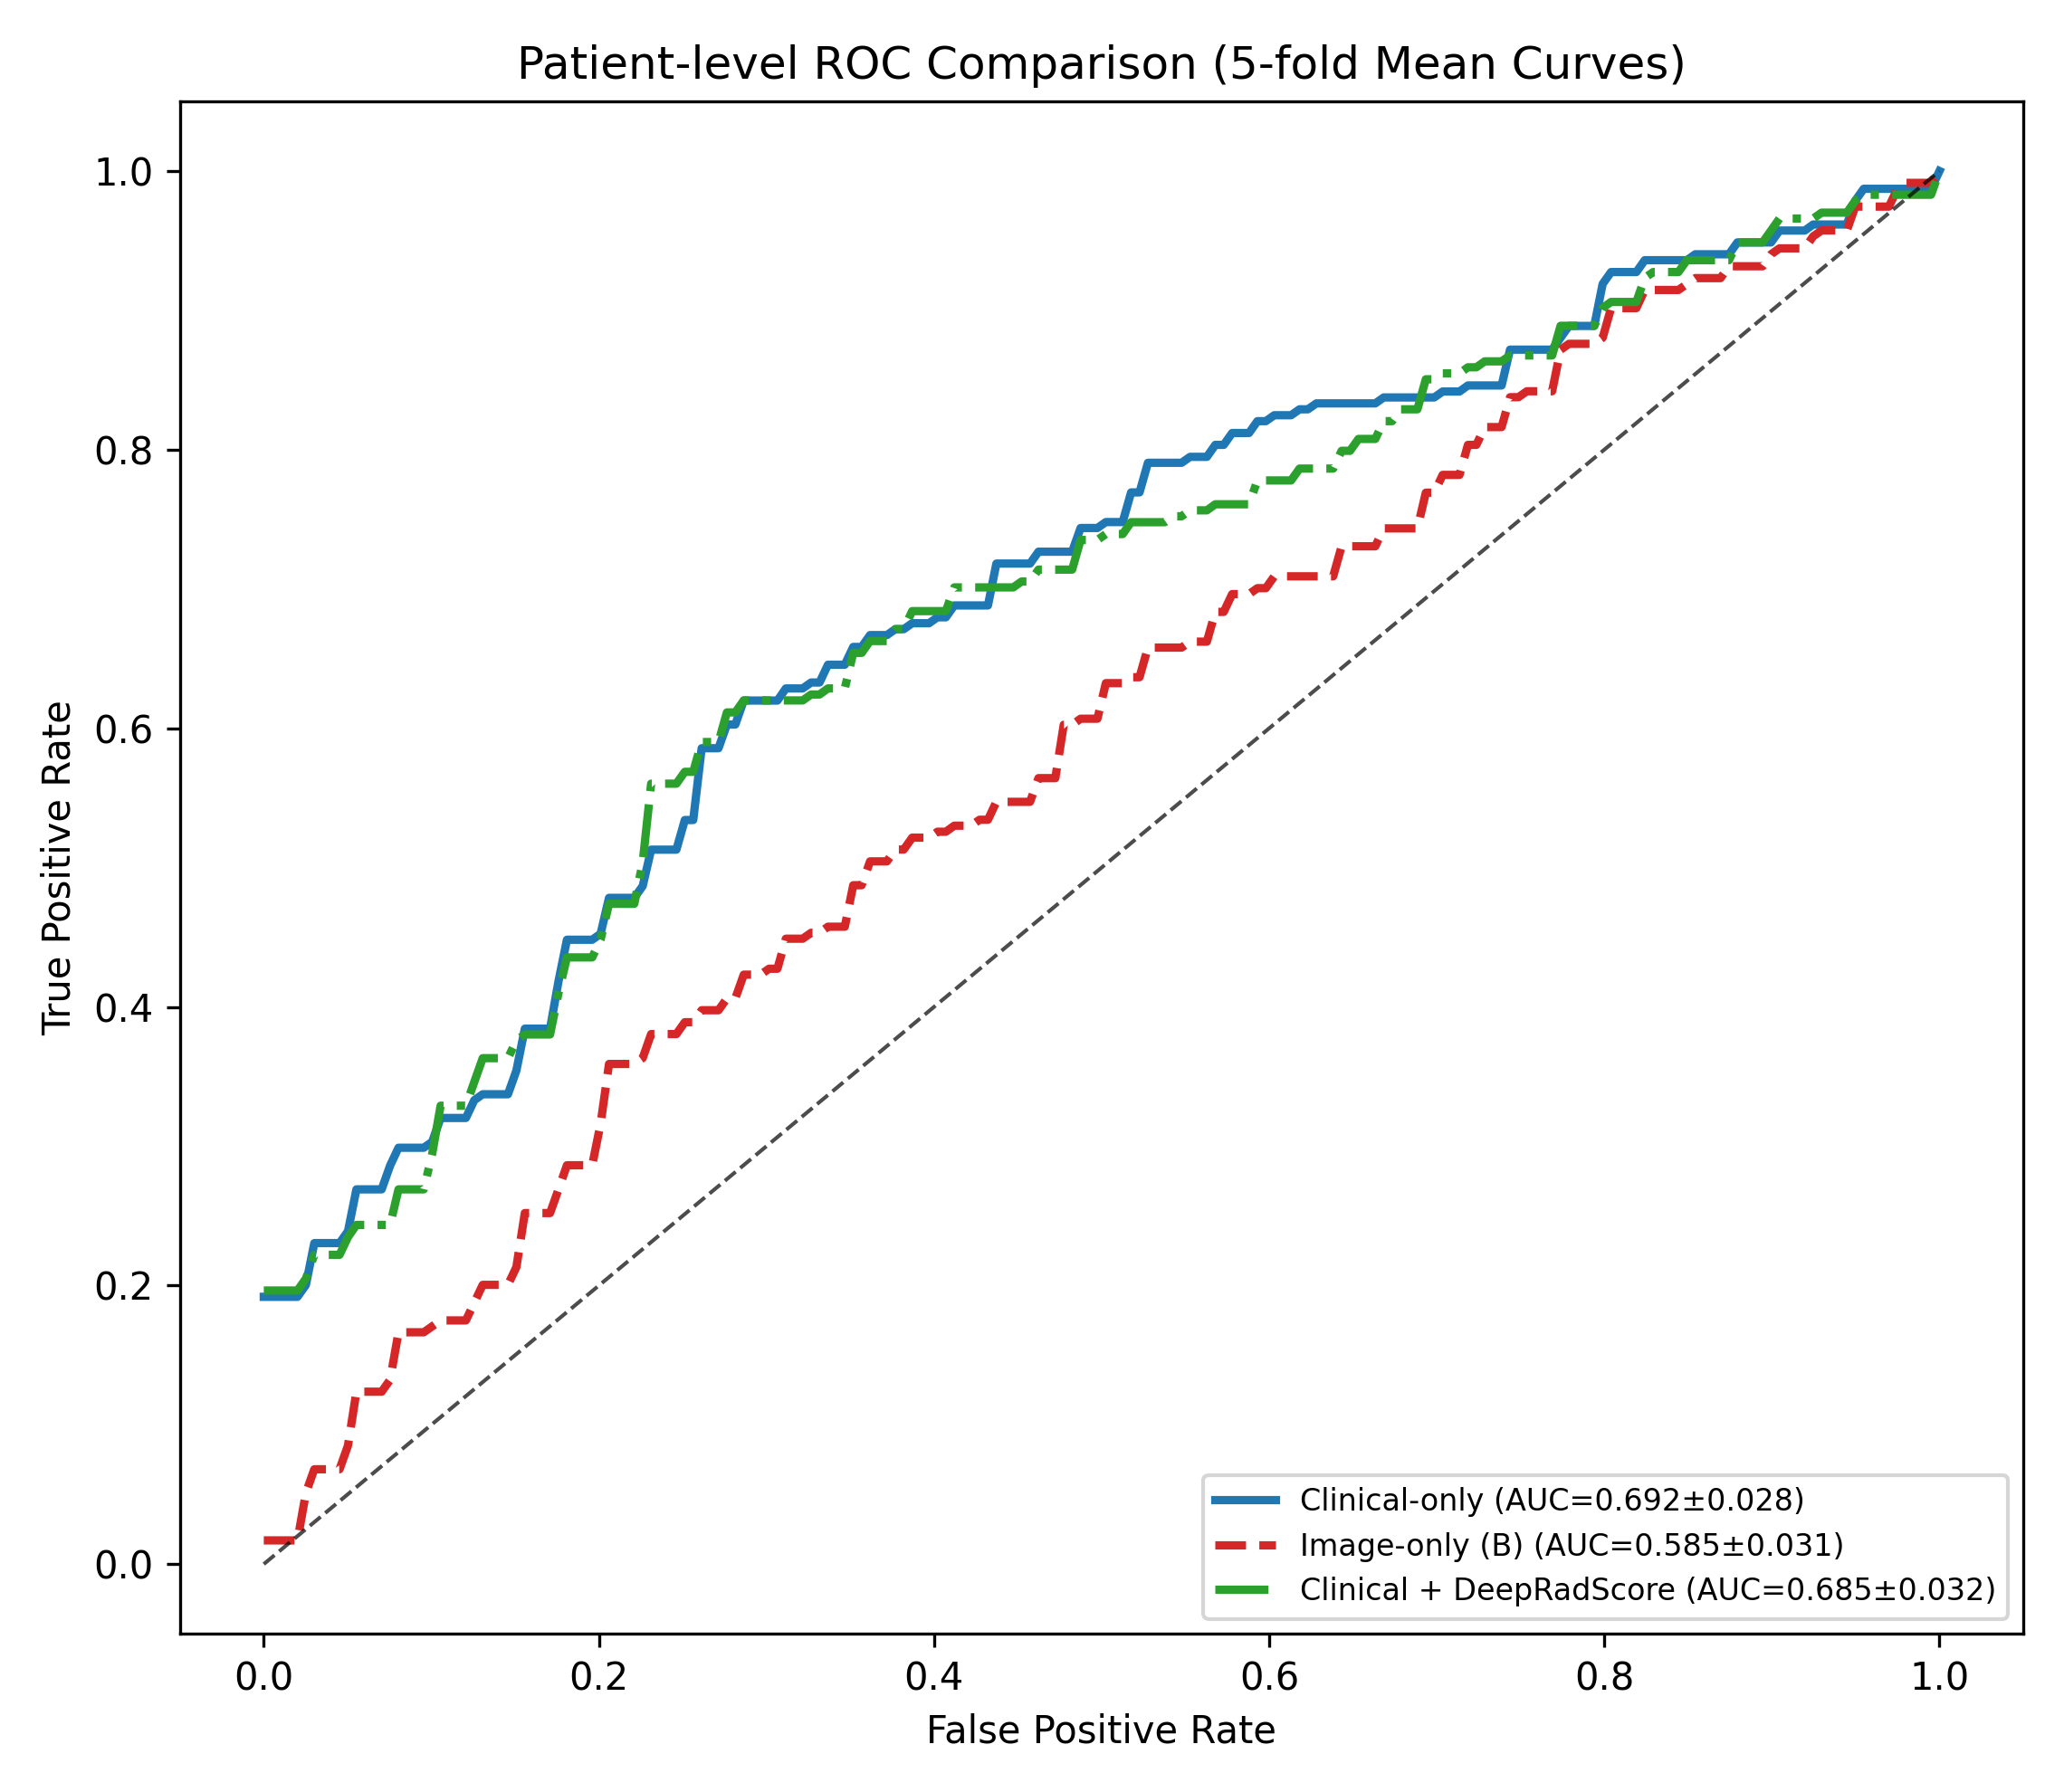
\includegraphics[width=0.78\textwidth]{figures/roc_overlay_three_routes.png}
  \caption{三路方法患者级 ROC 对比图（5-fold 均值曲线）。}
\end{figure}

\subsection{小结}
\begin{itemize}
  \item Clinical-only 在均值与稳定性上均明显优于 Image-only；
  \item Clinical+DeepRadScore 与 Clinical-only 接近，但没有持续且显著提升；
  \item 当前阶段结论：图像分支暂未提供稳健增益，可能引入额外噪声或域敏感性。
\end{itemize}

\section{实验 4：可解释性分析（病例级）}

\subsection{实验目的}
将“模型看哪里”和“哪个模块在推动预测”并行展示，解释三路对照结论在病例层面的表现。

\subsection{设置}
\begin{itemize}
  \item 选取代表性病例进行 Grad-CAM 热力图可视化；
  \item 同步展示模块贡献图（B / VUSE / VCEUS / Clinical）。
\end{itemize}

\subsection{定量表格}
\begin{table}[H]
\centering
\caption{可解释性分析观察要点}
\begin{tabular}{p{0.30\textwidth}p{0.62\textwidth}}
\toprule
维度 & 观察结论 \\
\midrule
空间关注（Grad-CAM） & 能提供局部关注区域，但跨病例一致性一般。 \\
模块贡献 & Clinical 模块贡献更稳定；图像模块贡献在不同病例间波动更大。 \\
与三路对照联动 & 与定量结果一致：图像特征目前更像“可解释但不稳定的辅助信号”。 \\
\bottomrule
\end{tabular}
\end{table}

\subsection{对应图}
\begin{figure}[H]
  \centering
  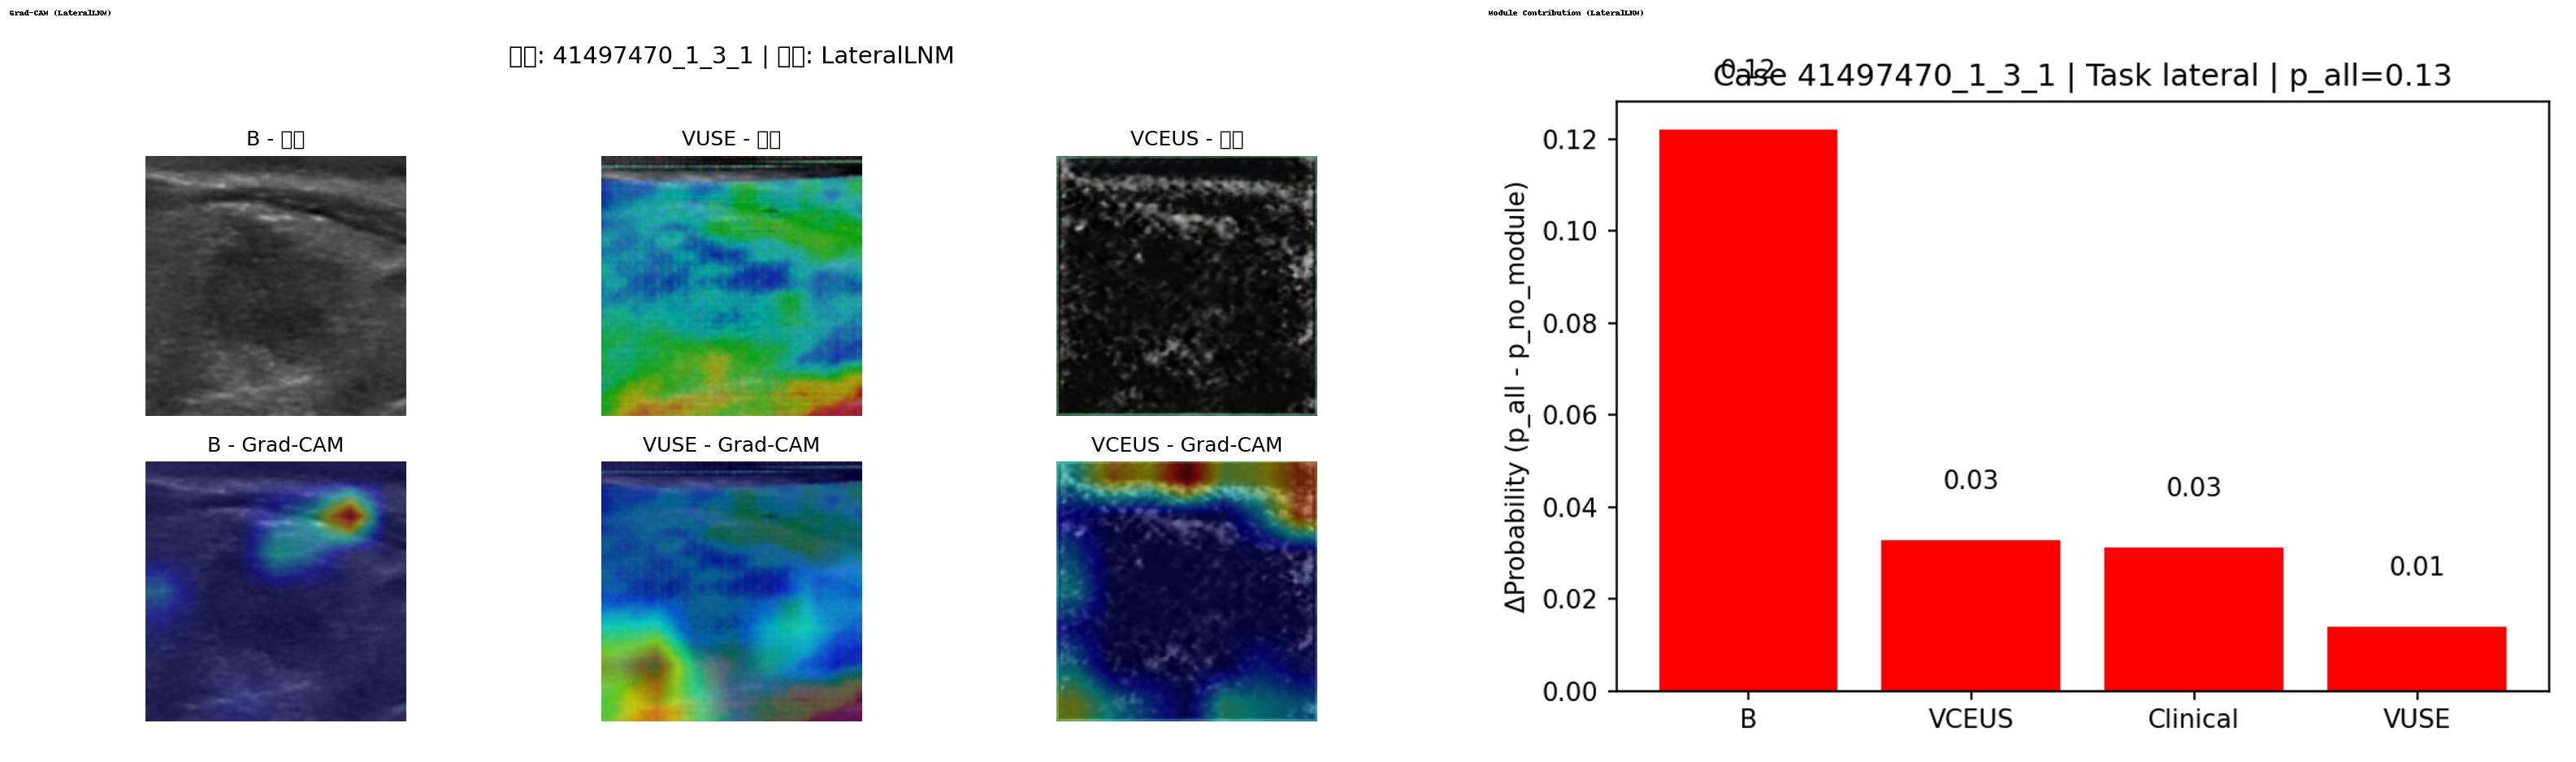
\includegraphics[width=0.95\textwidth]{figures/case_gradcam_module_panel.png}
  \caption{典型病例：Grad-CAM 与模块贡献并排图。}
\end{figure}

\subsection{小结}
\begin{itemize}
  \item 可解释性图支撑了定量结论：图像分支存在“个案可解释但群体不稳定”的现象；
  \item Clinical 信号在病例级和群体级都更稳定，适合作为当前阶段主路径。
\end{itemize}

\section{实验 5：传统影像组学多模型对照（患者级 5-fold）}

\subsection{实验目的}
在与深度学习实验一致的数据划分下，验证传统机器学习路线是否能提供可复现预测能力，并比较“临床-only / 影像组学-only / 临床+影像组学”三条 pipeline 的上限与稳定性。

\subsection{设置}
\begin{itemize}
  \item 数据与划分：沿用 \texttt{MultiModalDataset} 与 \texttt{groups\_cv5\_central} 的患者级 5-fold；
  \item 影像特征：B 模态图像的传统统计特征（强度直方图 + 一阶统计 + 梯度代理纹理），患者级 mean+max 聚合；
  \item Pipeline：\texttt{clinical\_only}、\texttt{radiomics\_only}、\texttt{clinical\_radiomics}；
  \item 模型池：LogReg、RandomForest、SVM(RBF)、AdaBoost、ExtraTrees、Stacking、SoftVoting（XGBoost 因环境缺包自动跳过）；
  \item 评估：统一报告 5-fold test 的 AUC 均值$\pm$标准差，并记录 ACC/F1/Sensitivity/Specificity。
\end{itemize}

\subsection{定量表格}
\begin{table}[H]
\centering
\caption{传统机器学习三条 pipeline 的全模型对照（5-fold test，按 AUC 均值排序）}
\begin{tabular}{llc}
\toprule
Pipeline & 模型 & AUC Mean$\pm$Std \\
\midrule
clinical-only & SoftVoting$^\star$ & 0.6894 $\pm$ 0.0486 \\
clinical-only & LogReg & 0.6877 $\pm$ 0.0456 \\
clinical-only & RandomForest & 0.6859 $\pm$ 0.0423 \\
clinical-only & Stacking & 0.6822 $\pm$ 0.0499 \\
clinical-only & ExtraTrees & 0.6607 $\pm$ 0.0544 \\
clinical-only & SVM(RBF) & 0.6485 $\pm$ 0.0468 \\
clinical-only & AdaBoost & 0.6438 $\pm$ 0.0449 \\
\midrule
clinical+radiomics & SoftVoting$^\star$ & 0.6862 $\pm$ 0.0314 \\
clinical+radiomics & Stacking & 0.6794 $\pm$ 0.0314 \\
clinical+radiomics & SVM(RBF) & 0.6738 $\pm$ 0.0343 \\
clinical+radiomics & LogReg & 0.6709 $\pm$ 0.0389 \\
clinical+radiomics & ExtraTrees & 0.6693 $\pm$ 0.0481 \\
clinical+radiomics & RandomForest & 0.6528 $\pm$ 0.0310 \\
clinical+radiomics & AdaBoost & 0.6271 $\pm$ 0.0241 \\
\midrule
radiomics-only & SoftVoting$^\star$ & 0.5831 $\pm$ 0.0156 \\
radiomics-only & Stacking & 0.5694 $\pm$ 0.0292 \\
radiomics-only & LogReg & 0.5684 $\pm$ 0.0204 \\
radiomics-only & SVM(RBF) & 0.5683 $\pm$ 0.0330 \\
radiomics-only & RandomForest & 0.5637 $\pm$ 0.0290 \\
radiomics-only & ExtraTrees & 0.5465 $\pm$ 0.0482 \\
radiomics-only & AdaBoost & 0.5357 $\pm$ 0.0284 \\
\bottomrule
\end{tabular}
\end{table}

\begin{table}[H]
\centering
\caption{每条 pipeline 的最佳模型（$^\star$）及辅助指标均值（5-fold test）}
\begin{tabular}{lccccc}
\toprule
Pipeline & 最佳模型 & AUC & ACC & F1 & Sen / Spe \\
\midrule
clinical-only & SoftVoting$^\star$ & 0.6894$\pm$0.0486 & 0.6285 & 0.6476 & 0.6329 / 0.6236 \\
clinical+radiomics & SoftVoting$^\star$ & 0.6862$\pm$0.0314 & 0.6264 & 0.6595 & 0.6668 / 0.5786 \\
radiomics-only & SoftVoting$^\star$ & 0.5831$\pm$0.0156 & 0.5870 & 0.6413 & 0.6834 / 0.4721 \\
\bottomrule
\end{tabular}
\end{table}

\subsection{对应图}
\begin{figure}[H]
  \centering
  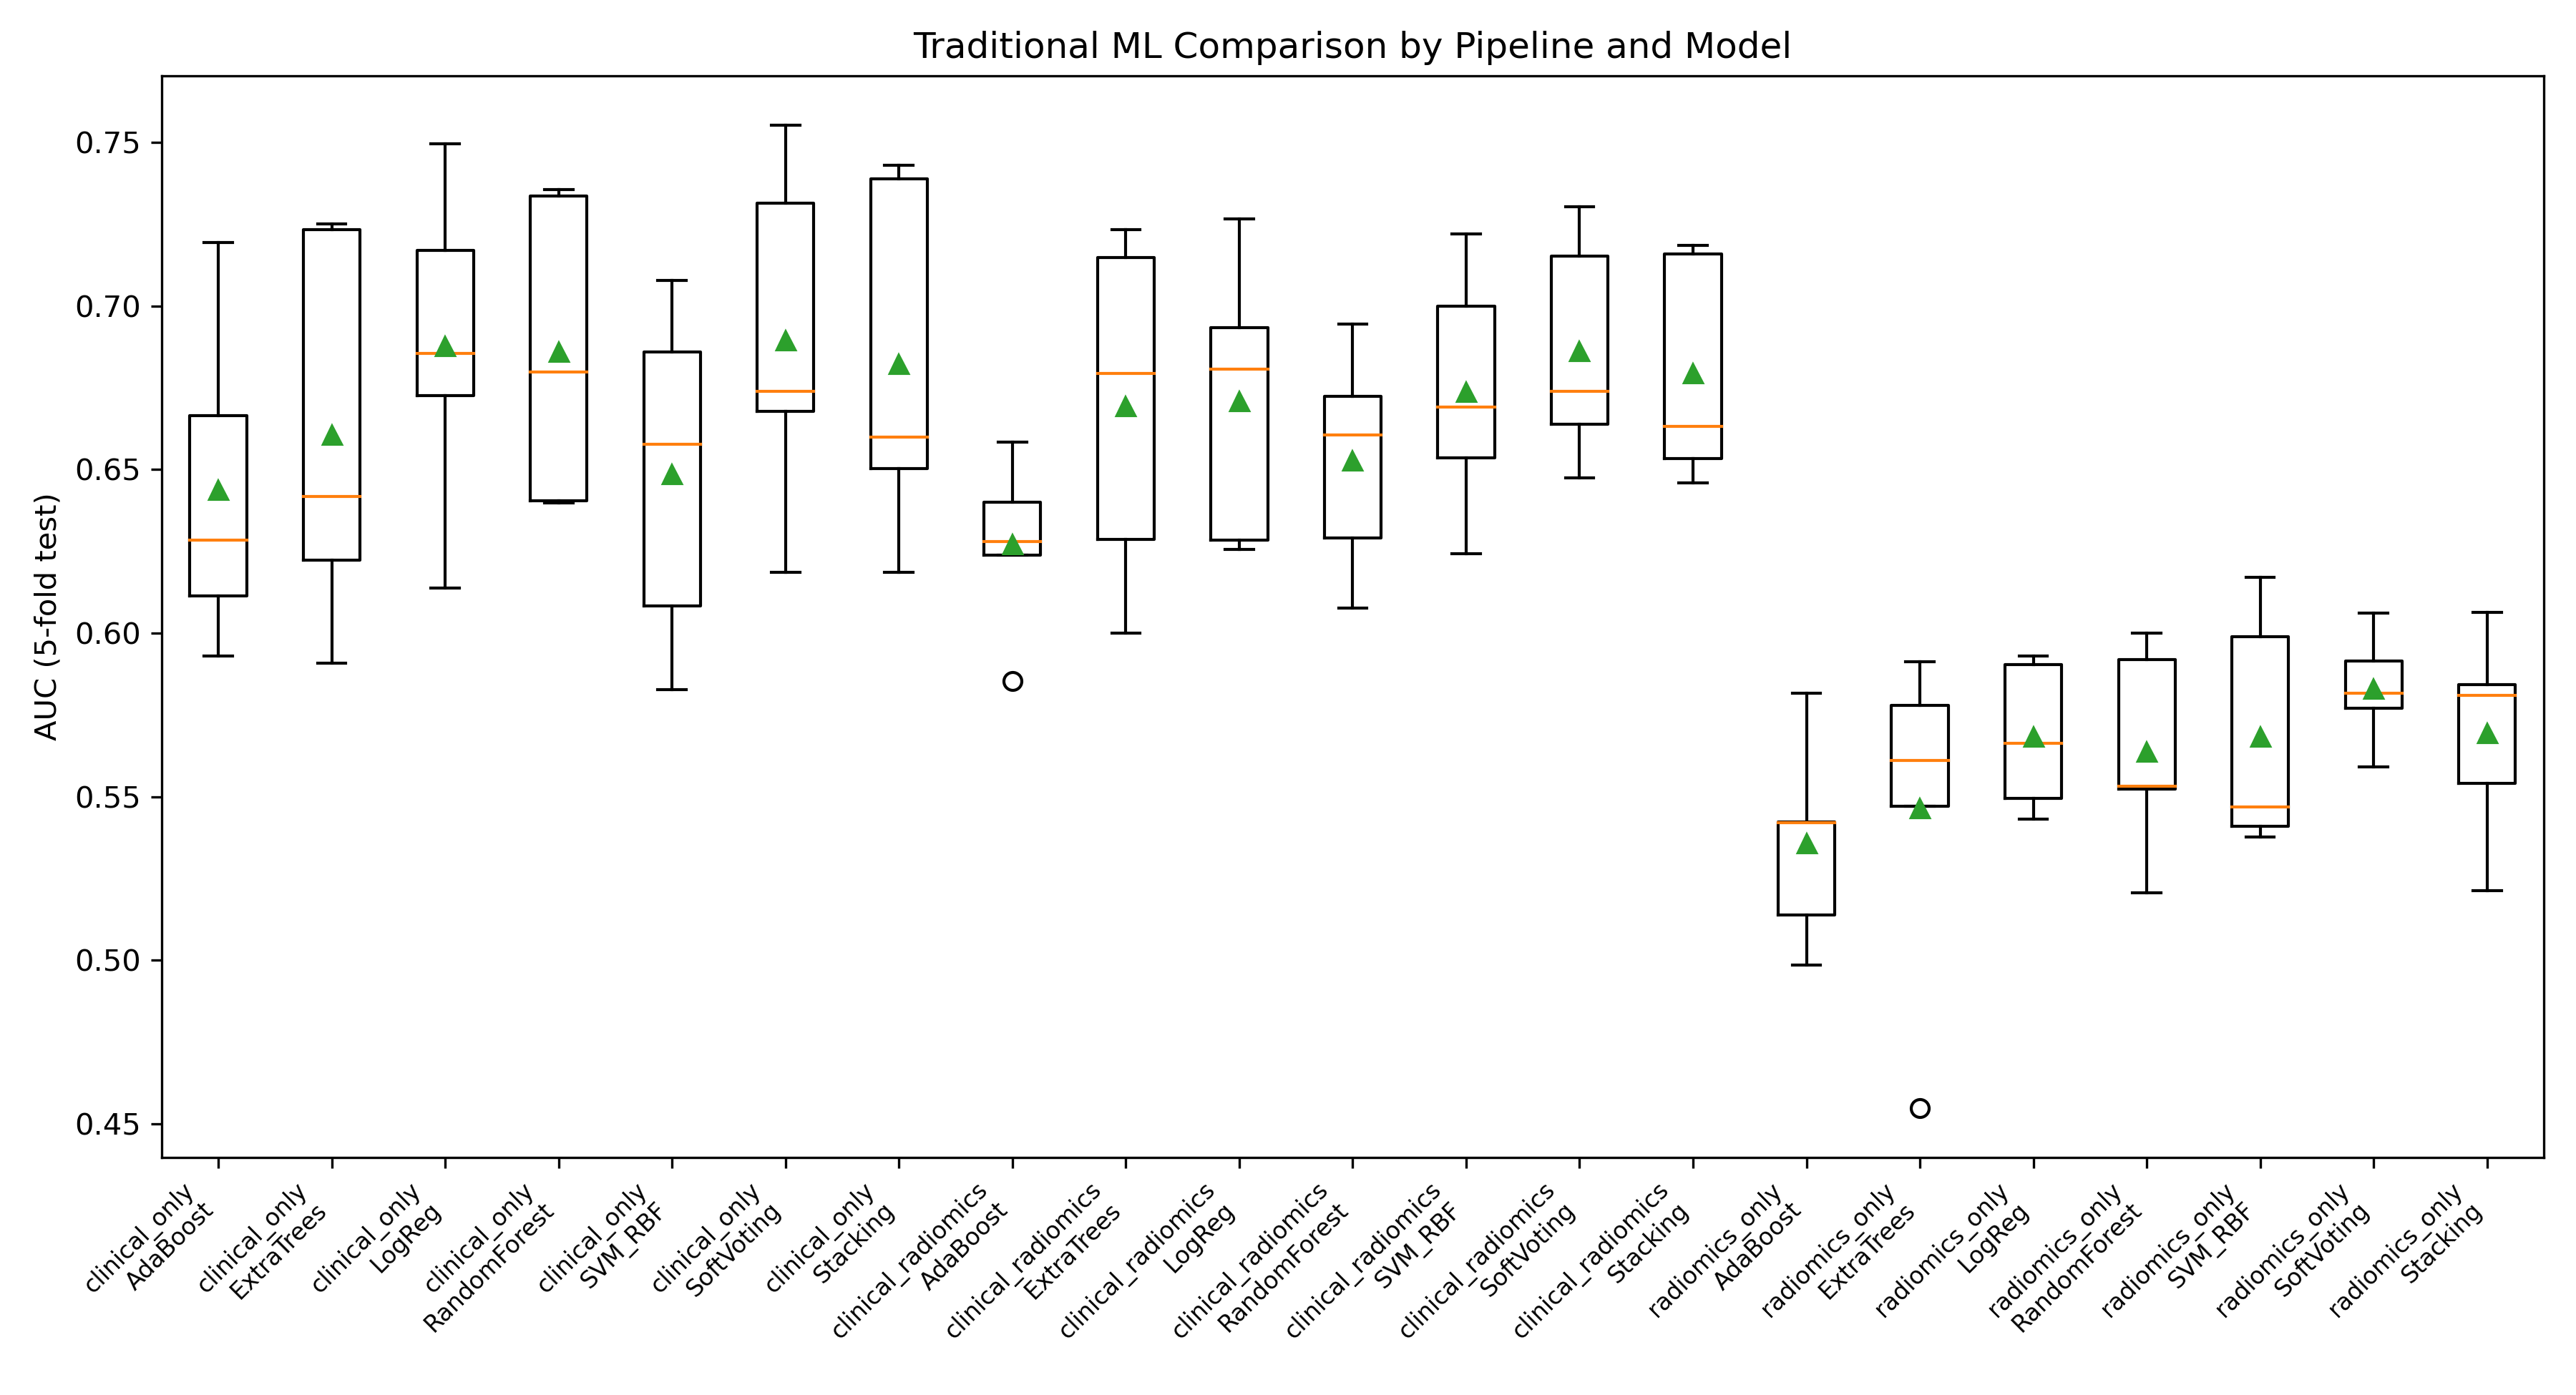
\includegraphics[width=0.90\textwidth]{figures/auc_boxplot_traditional_ml.png}
  \caption{传统机器学习：三条 pipeline 与多模型的 5-fold test AUC 箱线图。}
\end{figure}

\begin{figure}[H]
  \centering
  \begin{subfigure}[b]{0.32\textwidth}
    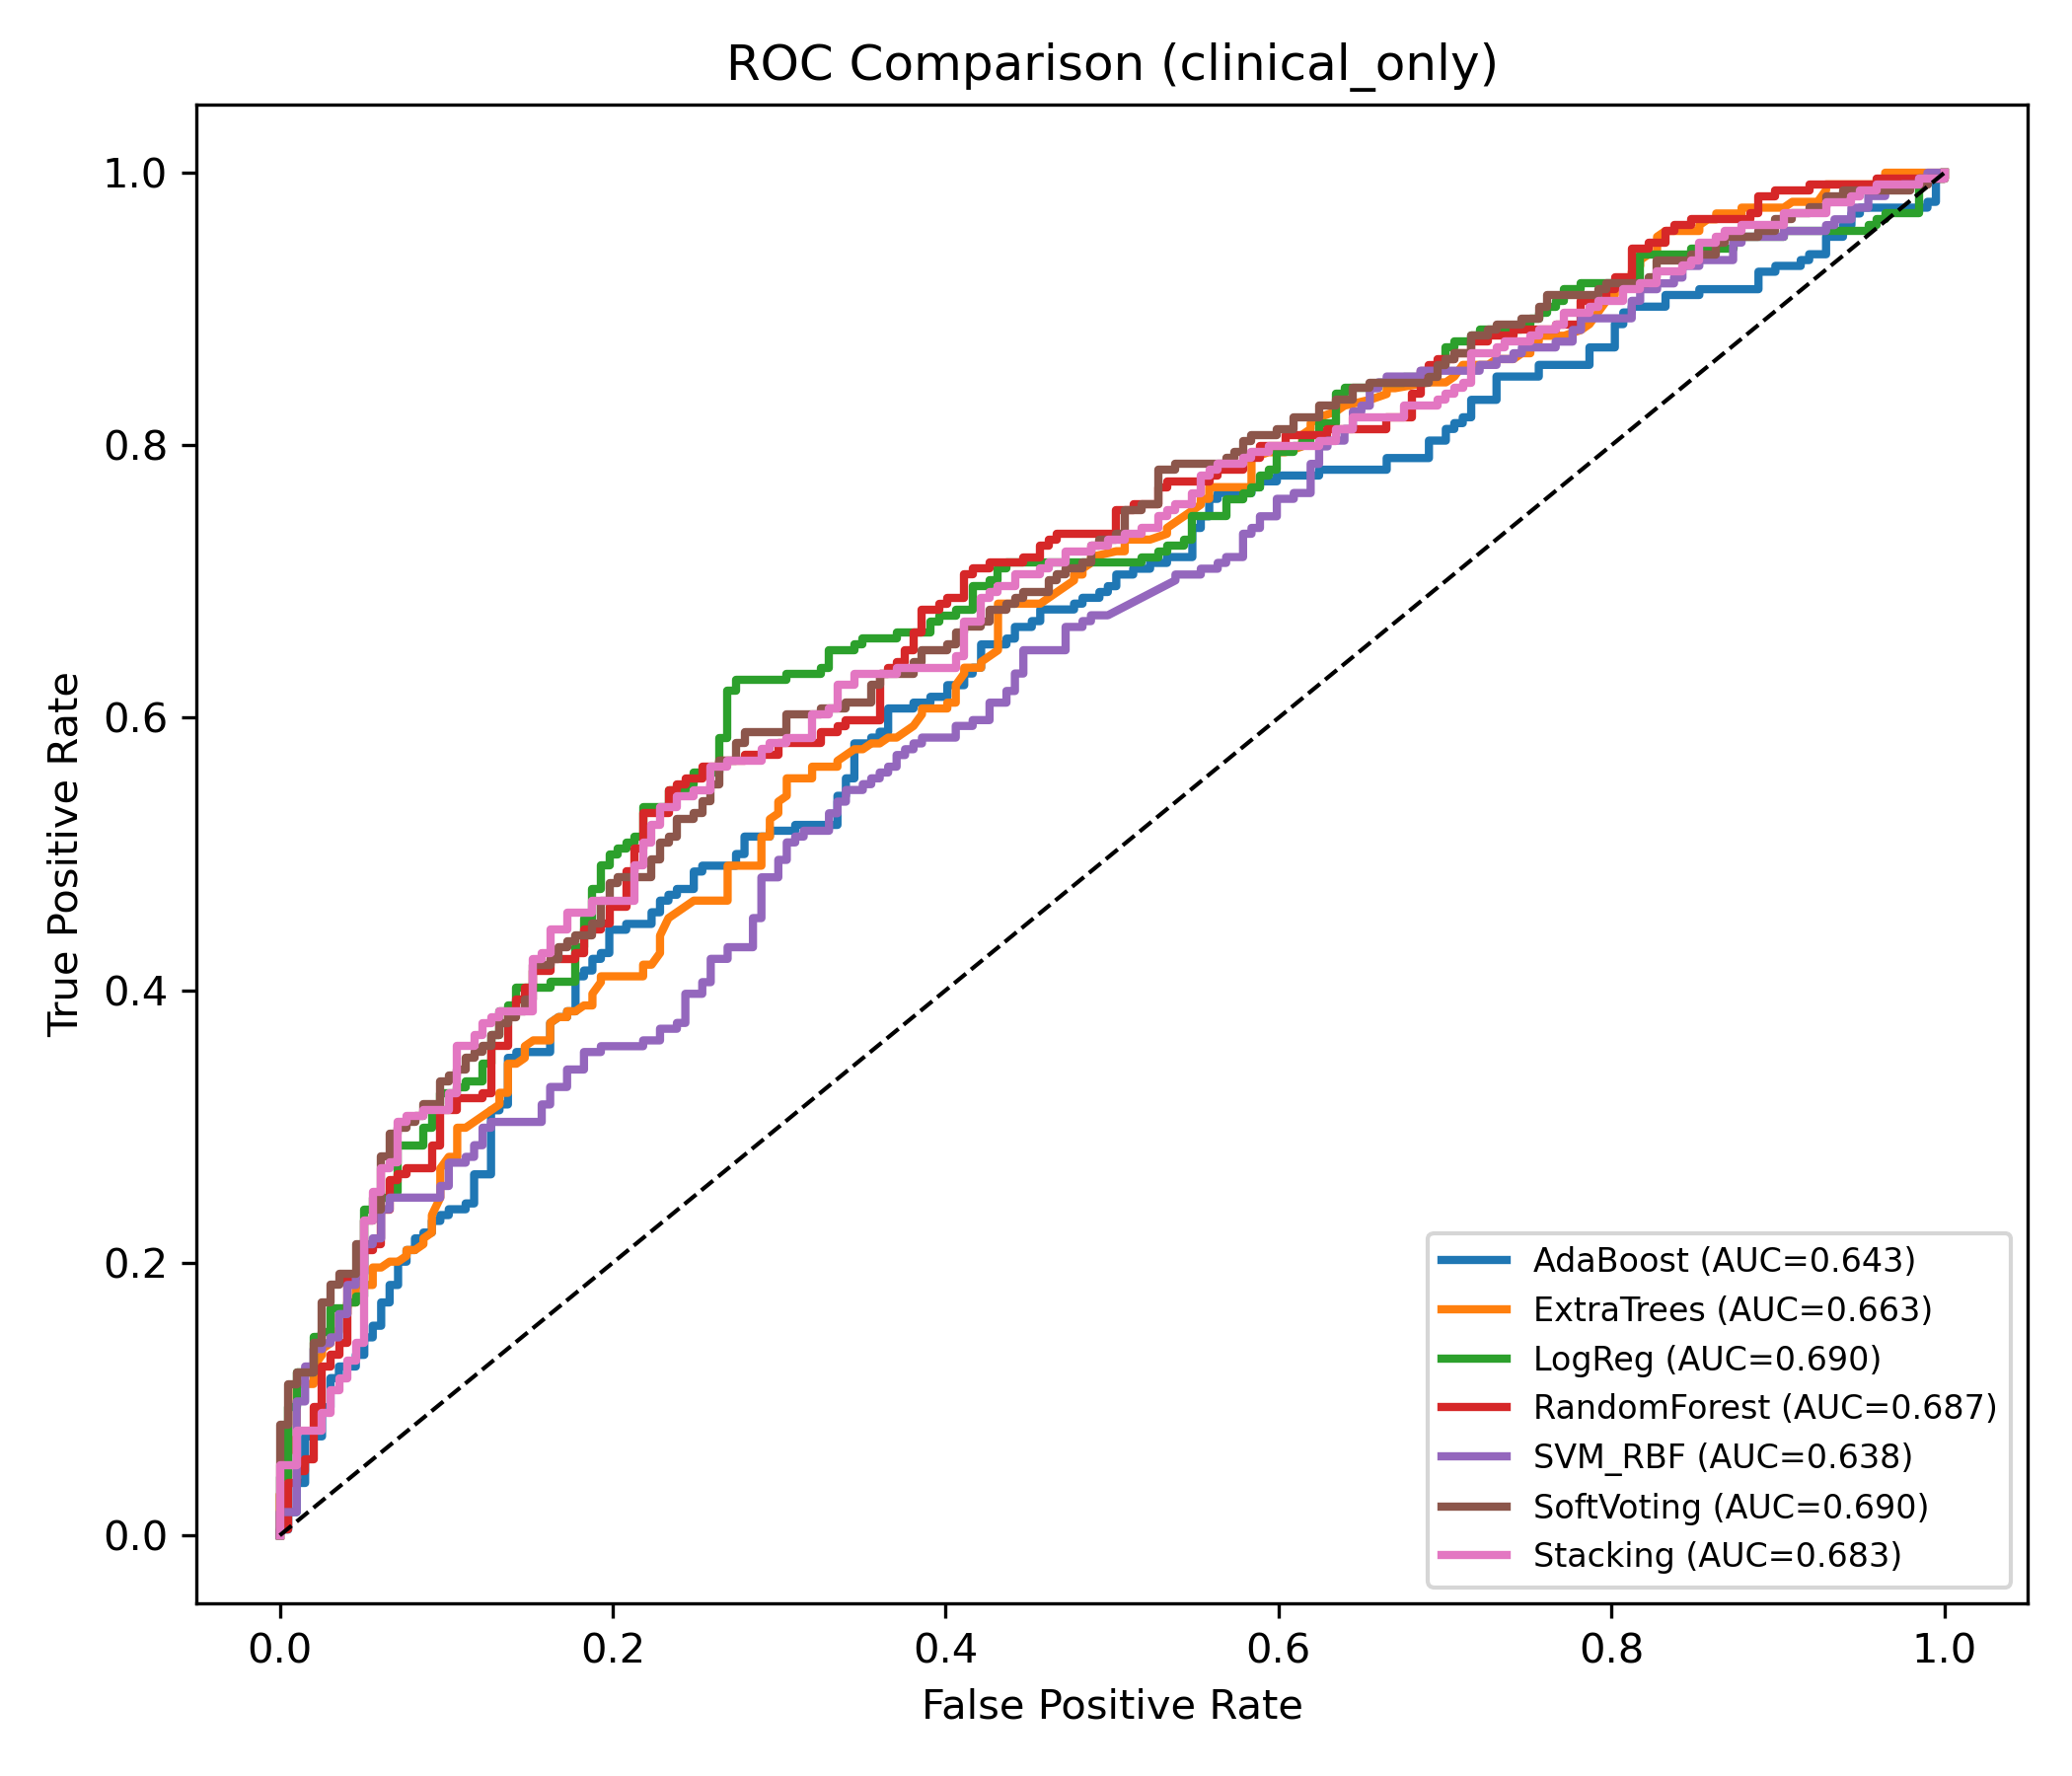
\includegraphics[width=\textwidth]{figures/roc_traditional_clinical_only.png}
    \caption{clinical-only}
  \end{subfigure}
  \begin{subfigure}[b]{0.32\textwidth}
    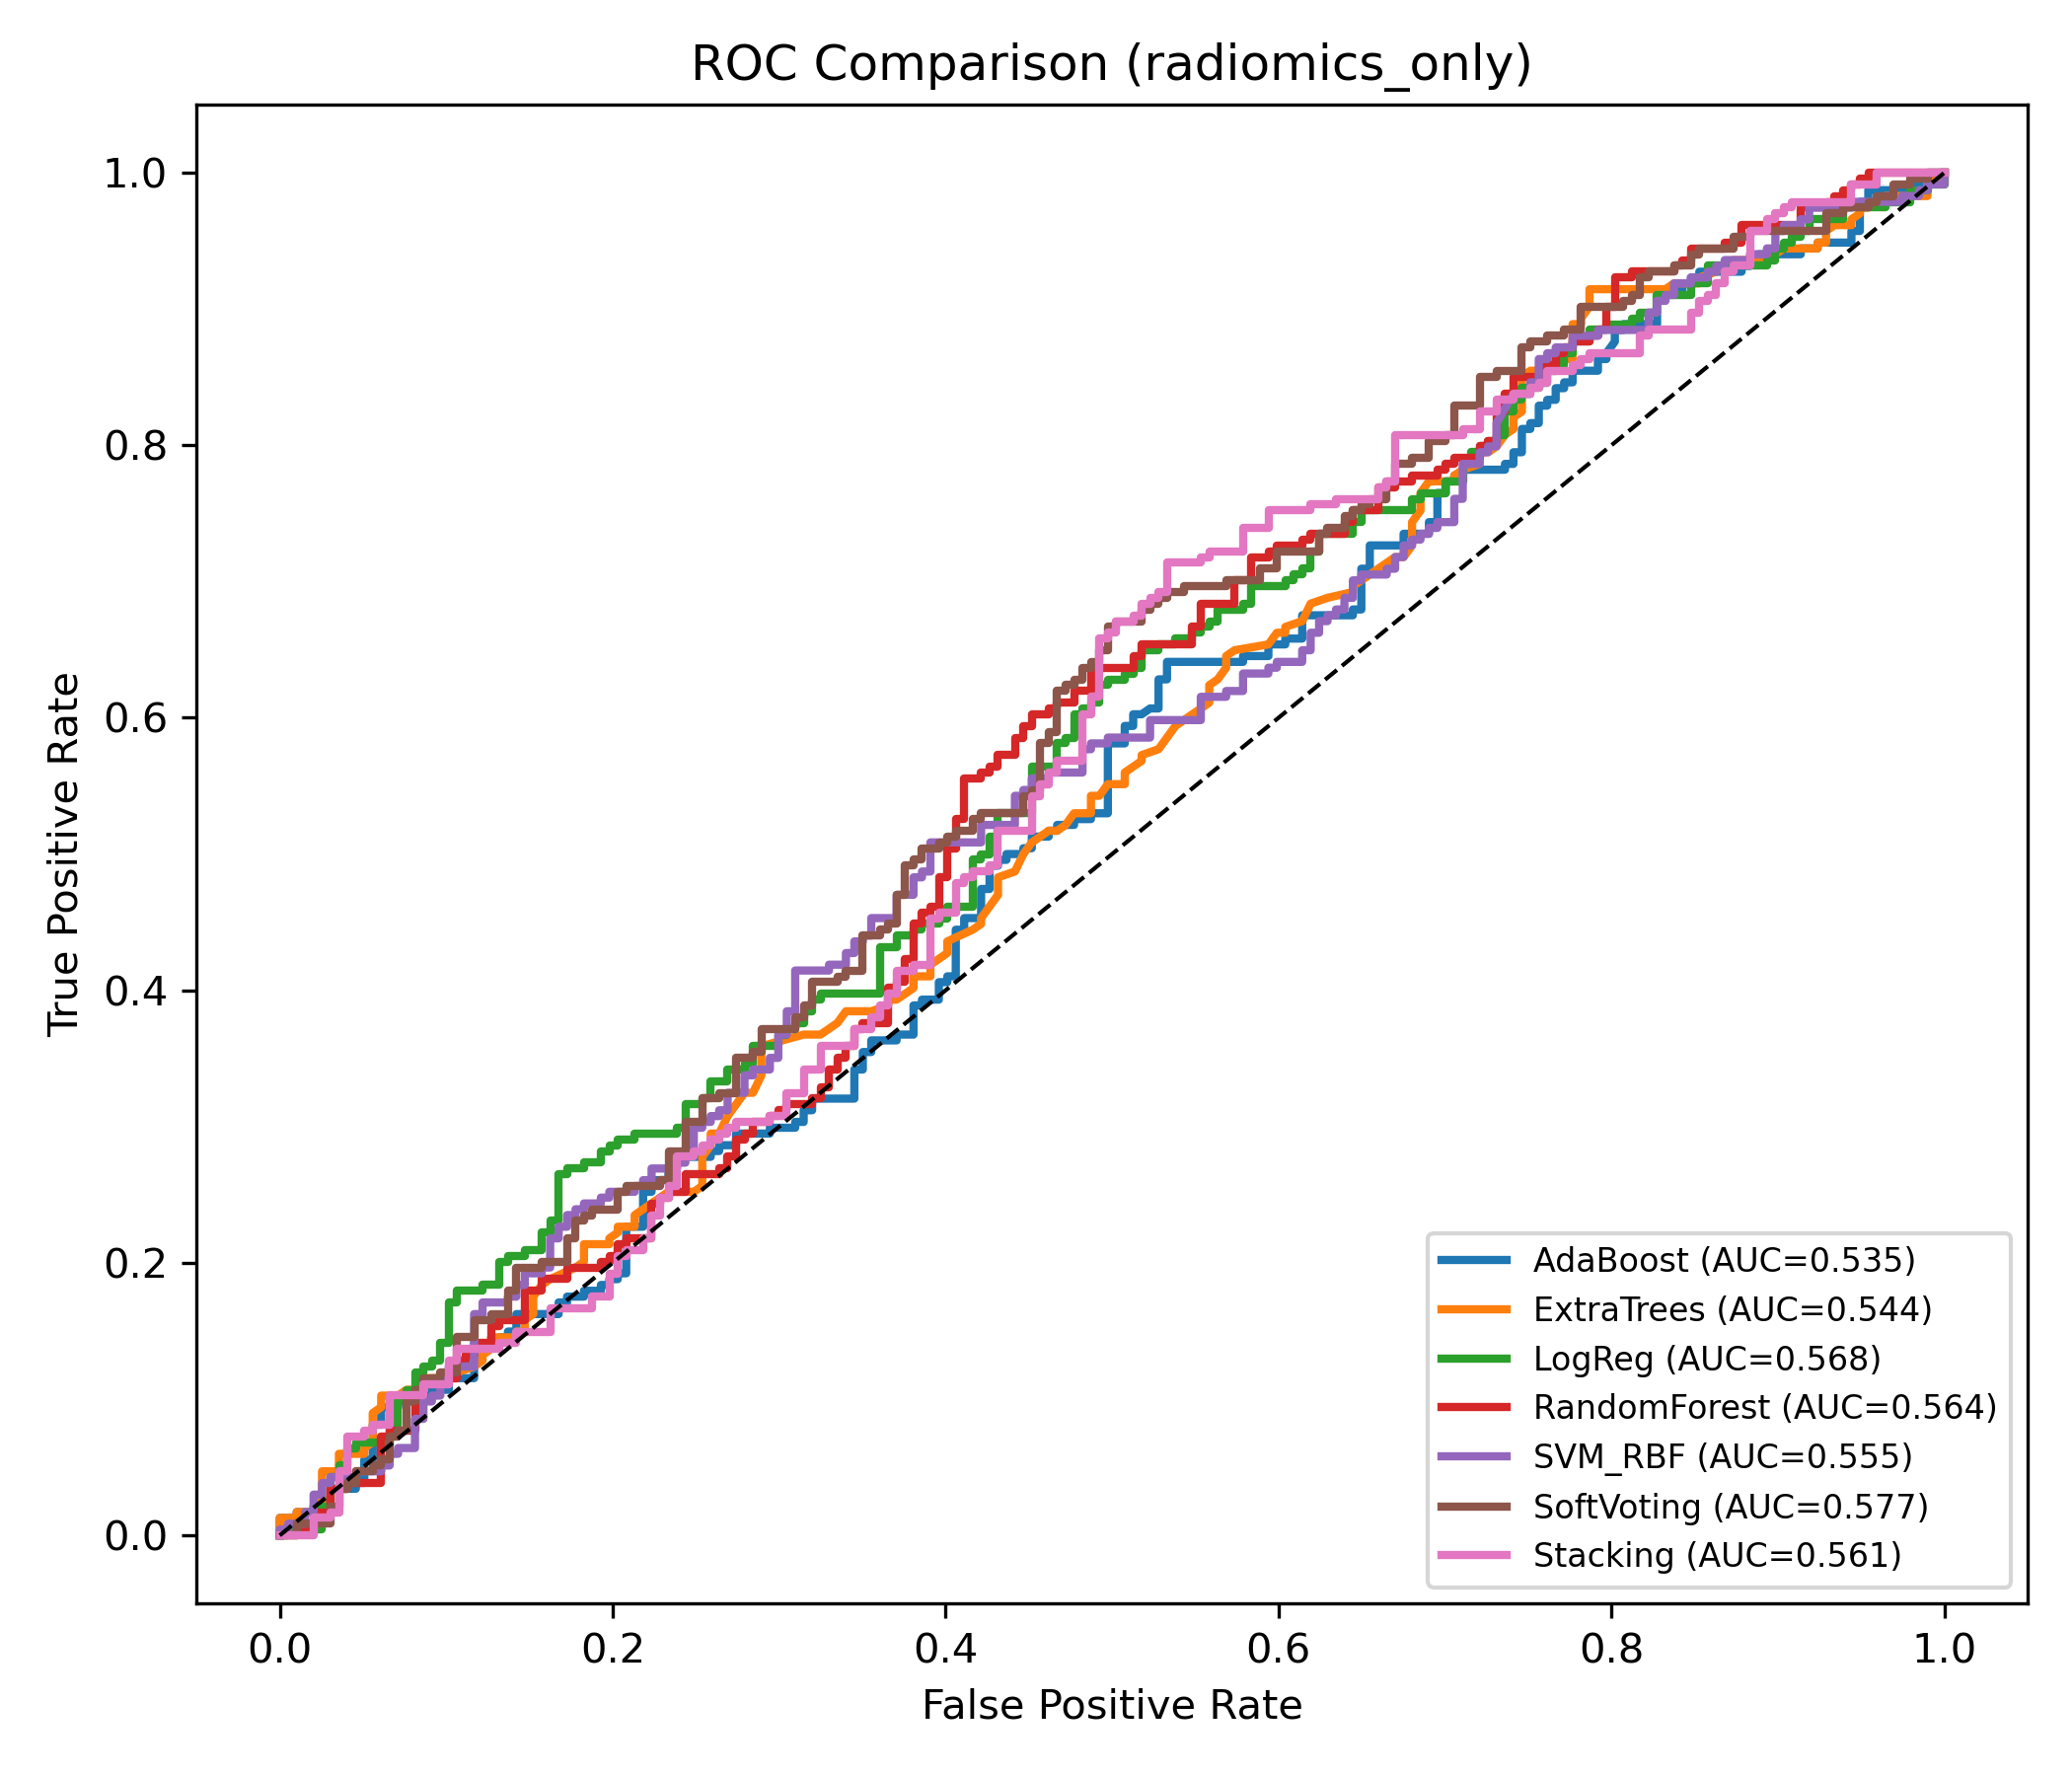
\includegraphics[width=\textwidth]{figures/roc_traditional_radiomics_only.png}
    \caption{radiomics-only}
  \end{subfigure}
  \begin{subfigure}[b]{0.32\textwidth}
    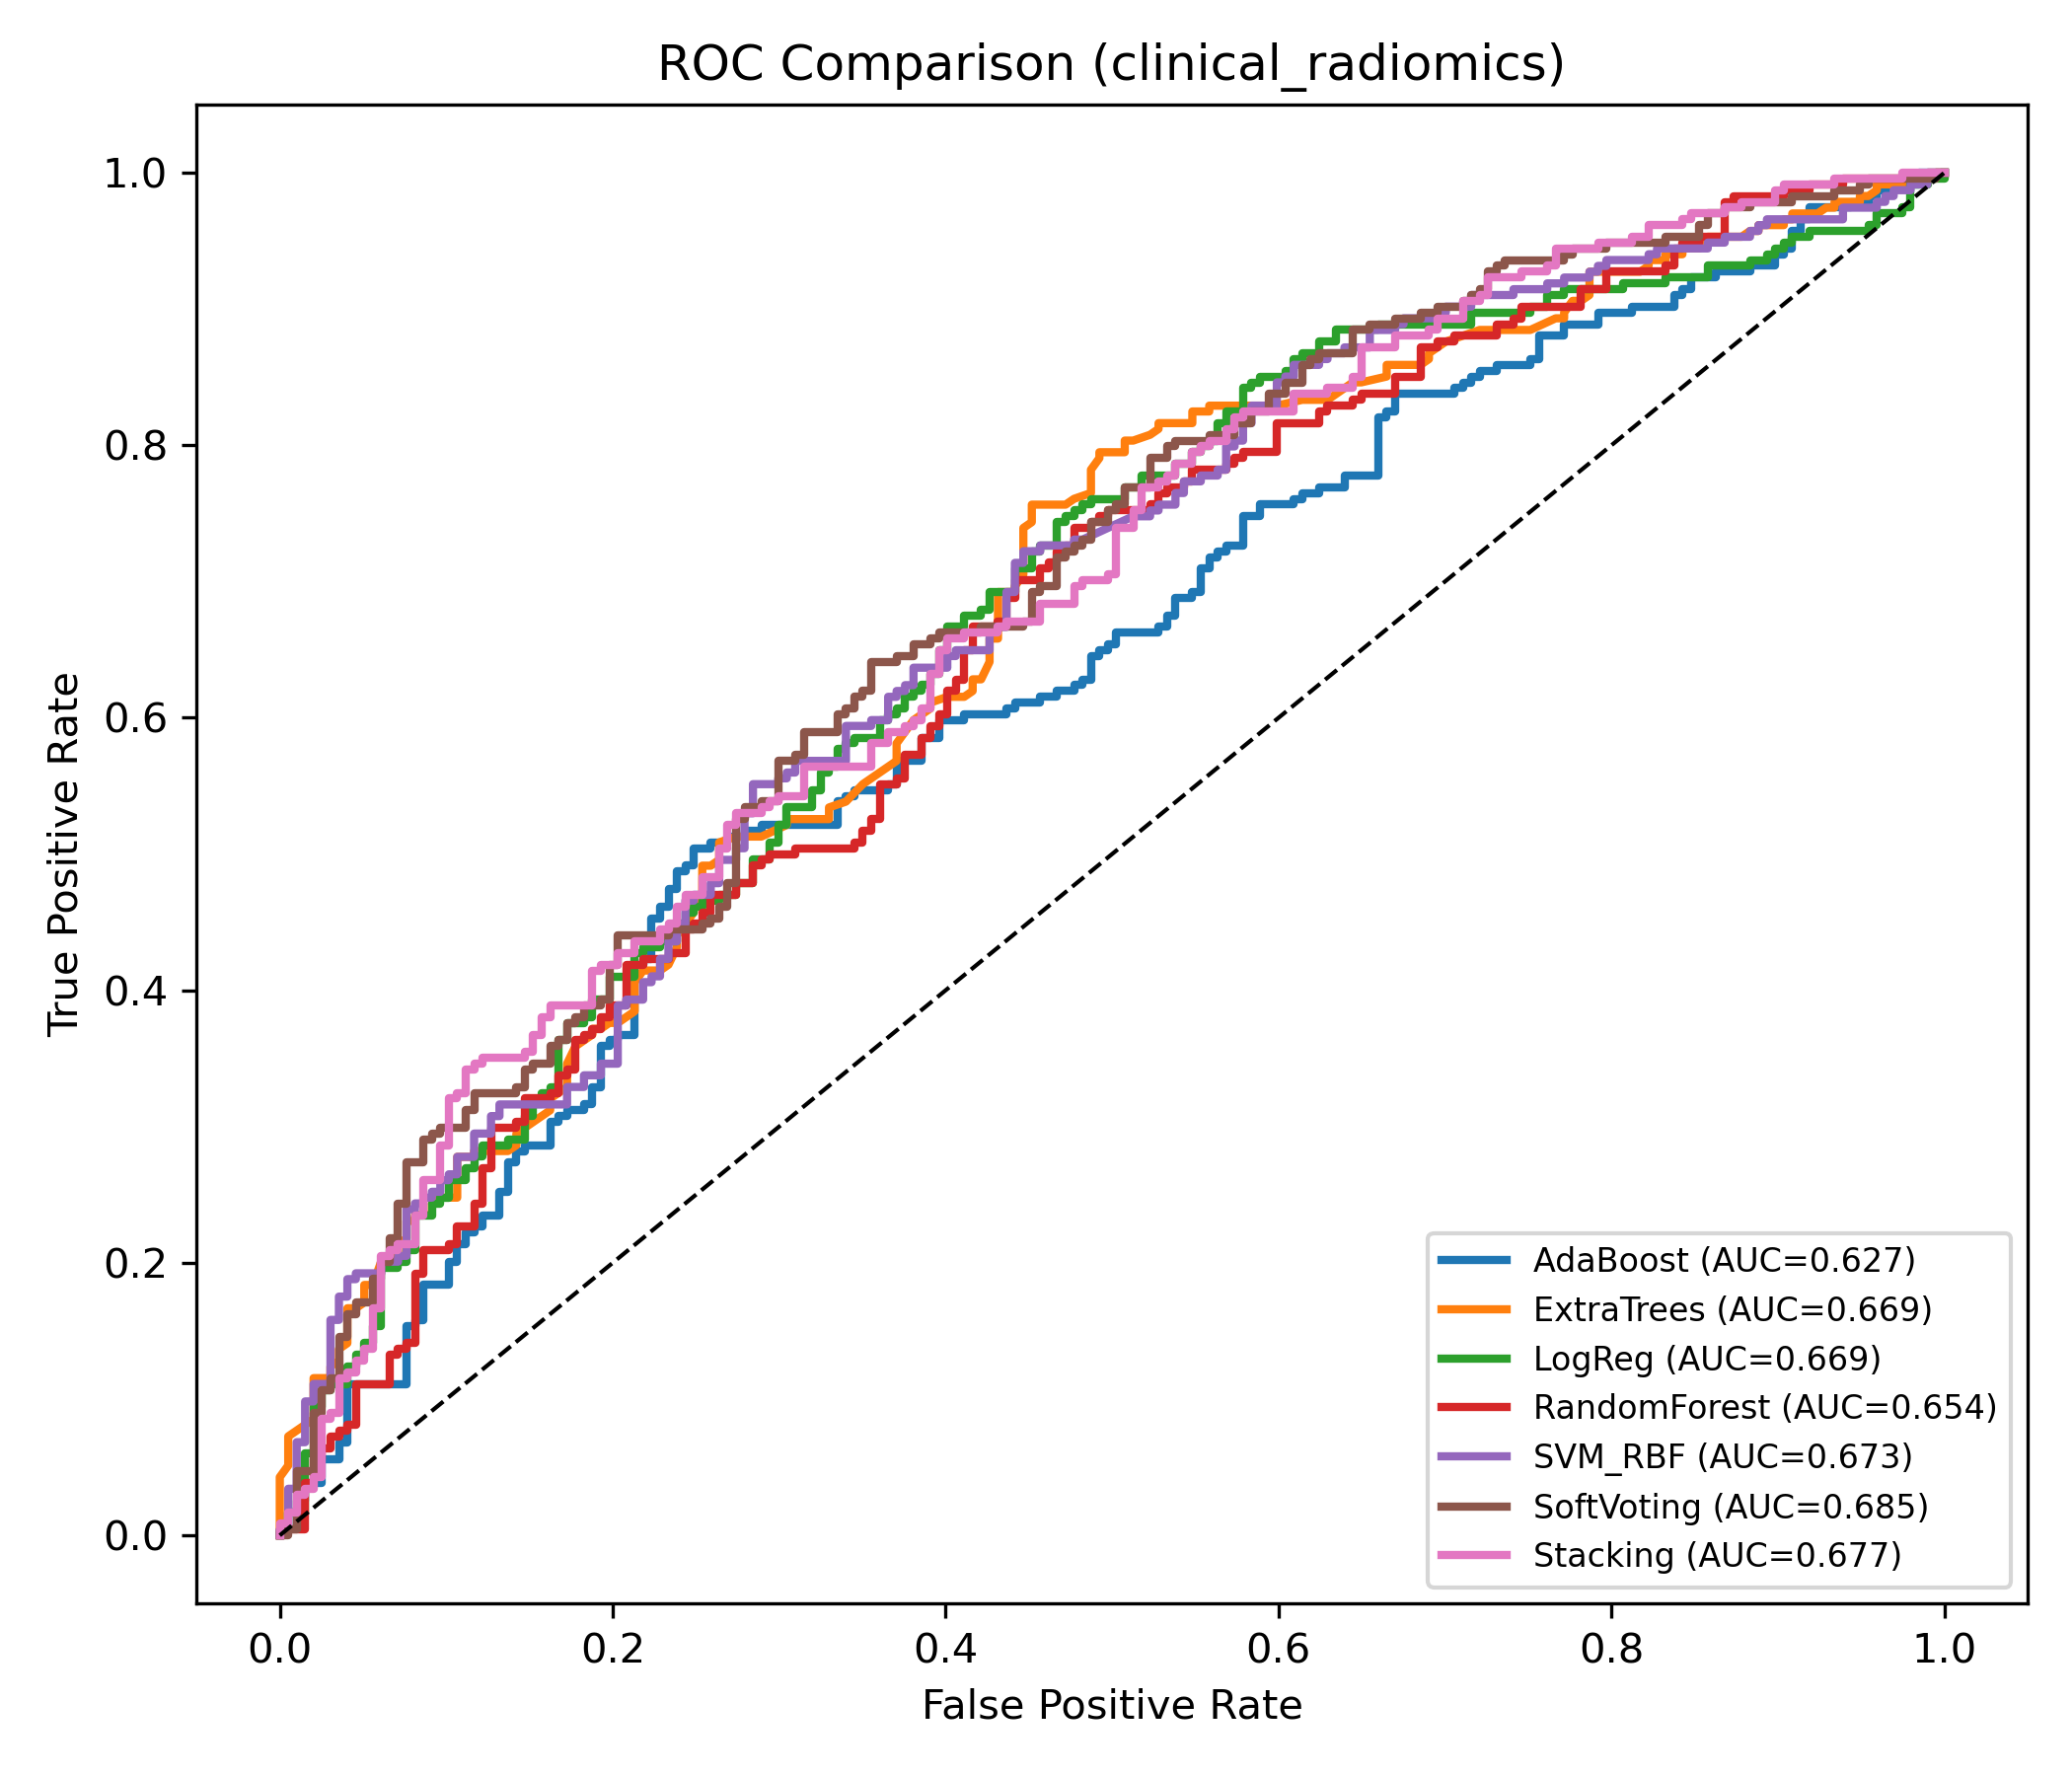
\includegraphics[width=\textwidth]{figures/roc_traditional_clinical_radiomics.png}
    \caption{clinical+radiomics}
  \end{subfigure}
  \caption{传统机器学习三条 pipeline 的多模型 ROC 对比图。}
\end{figure}

\subsection{小结}
\begin{itemize}
  \item 在传统机器学习范式下，\textbf{clinical-only 与 clinical+radiomics 几乎持平}，最佳均为 SoftVoting；
  \item radiomics-only 明显低于另外两条路径，提示当前影像统计特征单独可分性较弱；
  \item 全模型补齐后结论保持稳定：除个别折次波动外，融合路线总体仍未稳定超越临床基线；
  \item 临床与影像组学拼接未形成稳定超越，说明“影像信息可用但增益有限”的结论在传统范式下同样成立。
\end{itemize}


\section{实验 6：多模态 Attention-MIL 联合门控融合（6组消融，患者级 5-fold）}

\subsection{实验目的}
基于既往“影像分支增益不稳定”的结论，进一步验证三项关键设计是否有效：
(1) MIL 从切片级提升到患者级建模；
(2) 临床主导门控融合是否优于直接拼接；
(3) 先验约束损失（$P_{central}\le P_{lnm}$）是否提升逻辑一致性与稳定性。

\subsection{设置}
\begin{itemize}
  \item 数据与评估：沿用患者级 \texttt{groups\_cv5\_central}，统一 5-fold test 指标；
  \item 网络：共享实例编码器 +（Mean/Attention）MIL 聚合 +（Concat/Gated）融合 + 双头任务（LNM 与 CentralLNM）；
  \item 消融分组：Baseline A（clinical-only）、Baseline B（slice-mean-concat）、Ablation 1（mean-mil-gated）、Ablation 2（attention-mil-concat）、Ablation 3（full but $\alpha=0$）、Ours（full with $\alpha=1$）；
  \item 指标：CentralLNM 的 AUC/ACC/F1/Sensitivity/Specificity，以及逻辑依从率（Logical Compliance Rate）。
\end{itemize}

\subsection{定量表格}
\begin{table}[H]
\centering
\caption{实验 6：6组消融结果（CentralLNM，5-fold test）}
\begin{tabular}{lcc}
\toprule
设置 & AUC Mean$\pm$Std & Logical Compliance \\
\midrule
Baseline A：Clinical-only & 0.6674 $\pm$ 0.0327 & 0.7160 $\pm$ 0.1897 \\
Baseline B：Slice-level Mean Concat & 0.6710 $\pm$ 0.0252 & 0.6673 $\pm$ 0.1274 \\
Ablation 1：Mean-MIL + Gated & 0.6776 $\pm$ 0.0321 & 0.9954 $\pm$ 0.0049 \\
Ablation 2：Attention-MIL + Concat & 0.6673 $\pm$ 0.0293 & 0.9954 $\pm$ 0.0022 \\
Ablation 3：Full, $\alpha=0$ & 0.6720 $\pm$ 0.0252 & 0.5730 $\pm$ 0.1525 \\
\textbf{Ours：Attention-MIL + Gated + Prior} & \textbf{0.6963 $\pm$ 0.0115} & \textbf{0.9768 $\pm$ 0.0168} \\
\bottomrule
\end{tabular}
\end{table}

\subsection{对应图}
\begin{figure}[H]
  \centering
  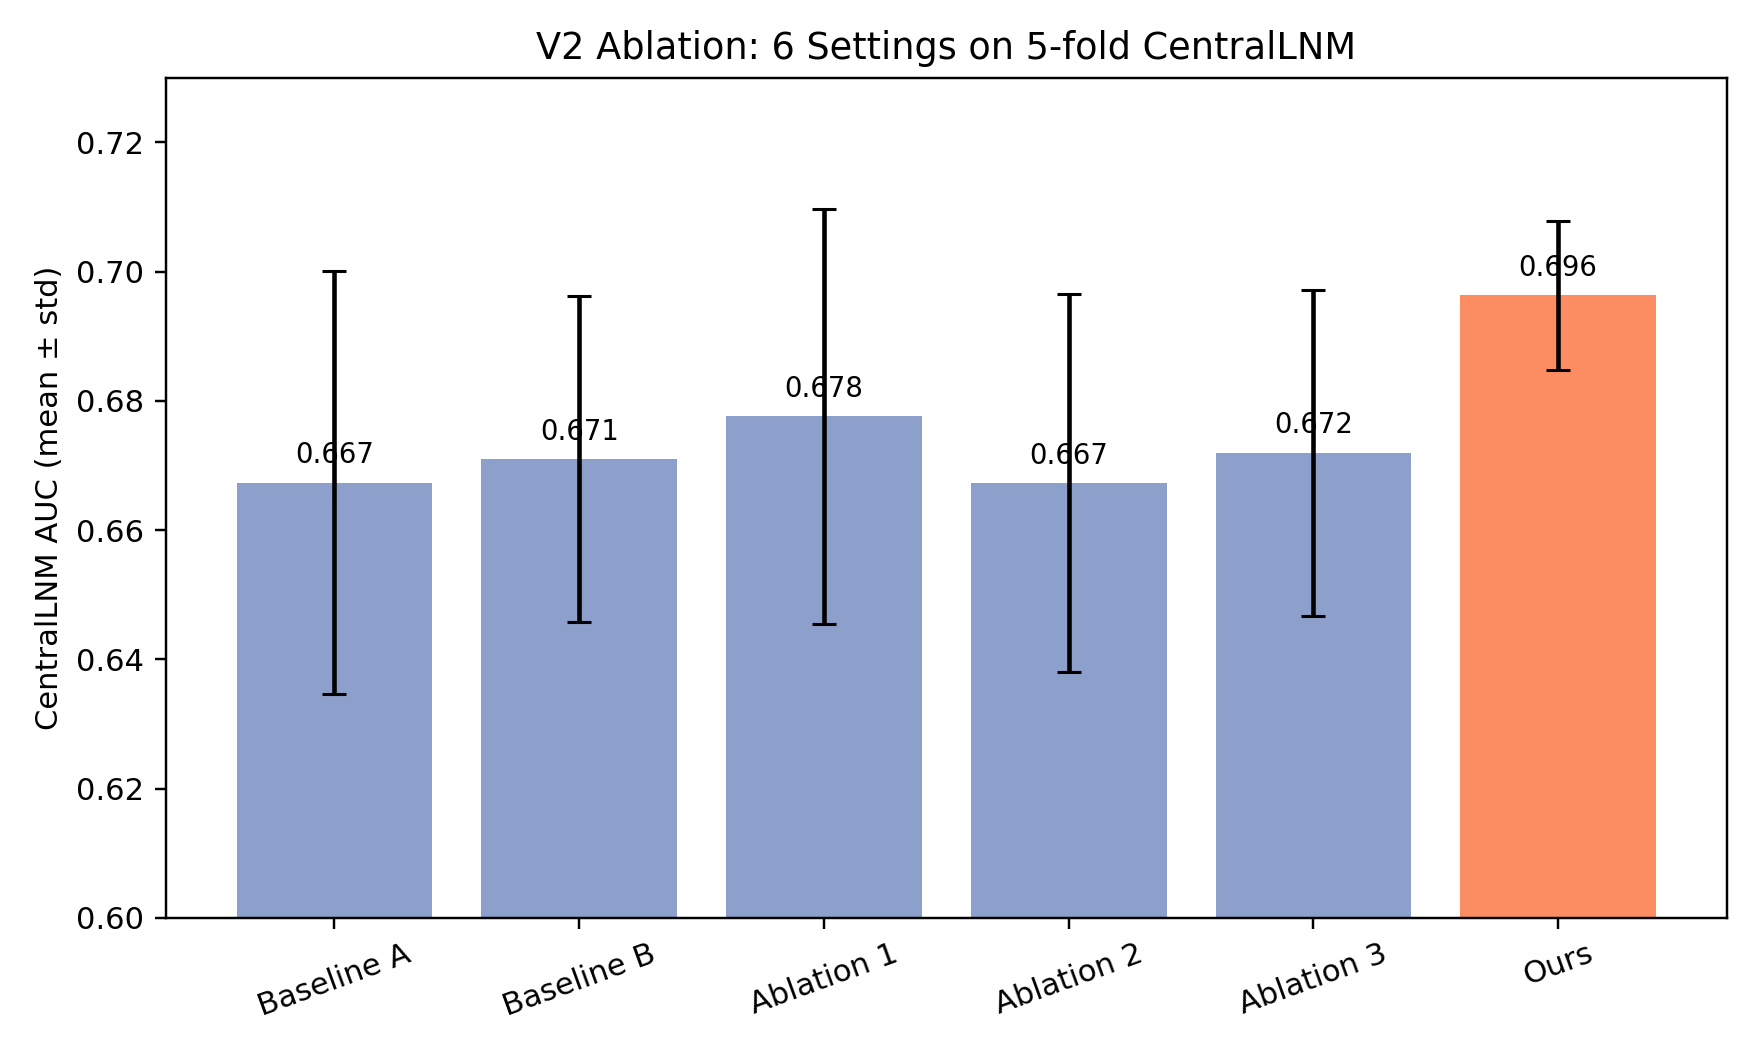
\includegraphics[width=0.85\textwidth]{figures/auc_bar_v2_ablation6.png}
  \caption{实验 6：6组消融在 CentralLNM 上的 AUC（5-fold mean$\pm$std）。}
\end{figure}

\begin{figure}[H]
  \centering
  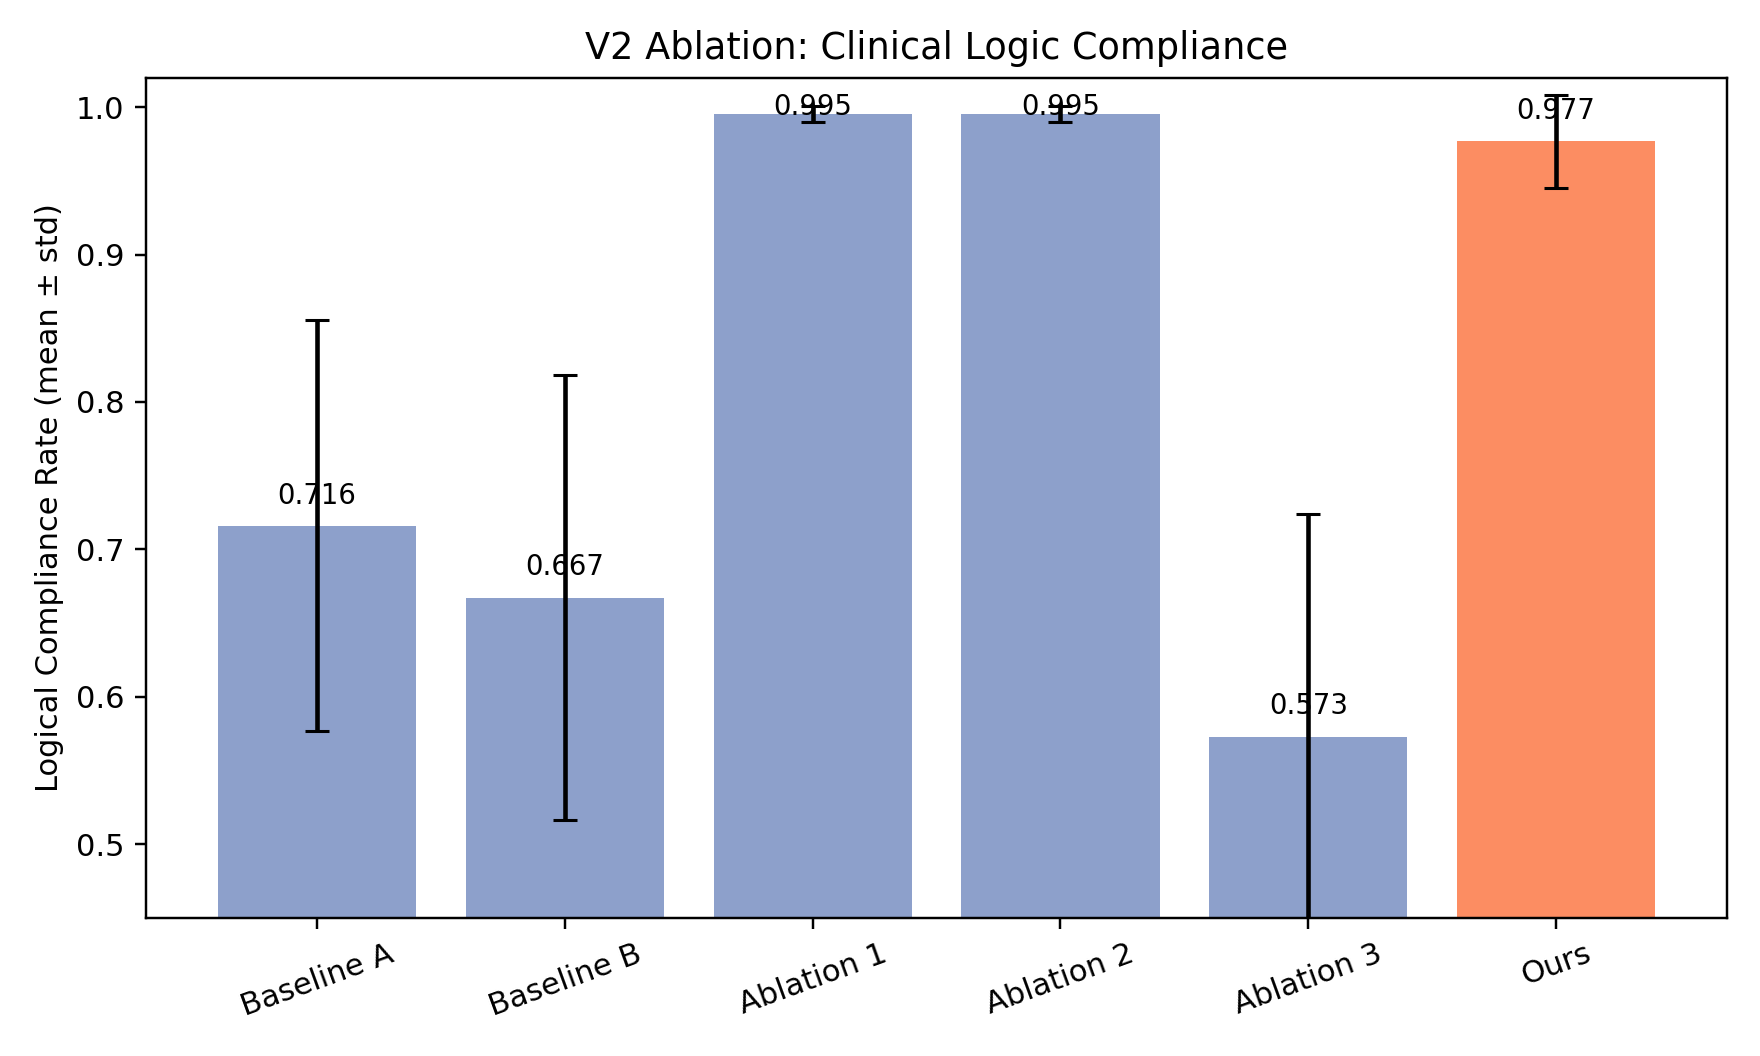
\includegraphics[width=0.85\textwidth]{figures/compliance_bar_v2_ablation6.png}
  \caption{实验 6：6组消融的临床逻辑依从率（$P_{central}\le P_{lnm}$）。}
\end{figure}

\subsection{小结}
\begin{itemize}
  \item \textbf{综合最优：}完整方案（Attention-MIL + Gated + Prior）达到最高 AUC（0.6963）且标准差最小（0.0115），说明增益不仅存在，而且更稳定；
  \item \textbf{门控价值：}在有 MIL 的条件下，门控融合（Ablation 1）较 concat 融合（Ablation 2）表现更优，支持“临床主导过滤影像噪声”的设计；
  \item \textbf{先验约束价值：}去掉先验（Ablation 3）后逻辑依从率显著下降（0.5730），加入先验后可稳定维持高依从率（Ours 0.9768）；
  \item 与前文深度三路和传统组学结果一致：临床信号仍是下限保障，但通过患者级 MIL + 门控 + 先验可实现更稳健的融合提升。
\end{itemize}

\section{实验 7：三源融合续跑（ROI Radiomics + Deep MIL + Clinical Gated）}

\subsection{实验目的}
在既有实验基础上完成“临床 + 深度学习 + 传统组学”一体化验证，重点回答两点：
(1) 标准 ROI Radiomics（非无分割统计特征）能否在患者级带来稳定信息；
(2) 将 Radiomics 作为影像分支补充后，三源门控融合（Ours V2）是否优于深度双源（Ours V1）。

\subsection{设置}
\begin{itemize}
  \item 数据划分：沿用患者级 \texttt{groups\_cv5\_central}，统一 5-fold test；
  \item 阶段 1（Baseline C/D）：B 模态原图 + 原始 mask 的 ROI Radiomics，患者级 mean+max 聚合，训练集内 LASSO 筛选（保留低维核心特征）；
  \item 阶段 2（Ours V1）：EffNet-B0 + Attention-MIL + Clinical Gated，\texttt{pretrained=True}，冻结前 3 epoch 后解冻；
  \item 阶段 3（Ours V2）：在 Ours V1 基础上加入患者级 ROI Radiomics 分支（Tri-Fusion），其余训练协议保持一致；
  \item 指标：AUC/ACC/F1/Sensitivity/Specificity 与 Logical Compliance。
\end{itemize}

\subsection{定量表格}
\begin{table}[H]
\centering
\caption{实验 7：三源阶段核心结果汇总（CentralLNM，5-fold test）}
\begin{tabular}{lcccccc}
\toprule
设置 & AUC Mean$\pm$Std & ACC & F1 & Sen & Spe & Compliance \\
\midrule
Baseline C: Radiomics-only（LogReg） & 0.5756 $\pm$ 0.0538 & 0.5566 & 0.6151 & 0.6536 & 0.4417 & -- \\
Baseline D: Clinical+Radiomics（SoftVoting） & \textbf{0.6923 $\pm$ 0.0696} & 0.6330 & 0.6672 & 0.6839 & \textbf{0.5729} & -- \\
Ours V1: Deep MIL + Clinical Gated（EffNet-B0） & 0.6732 $\pm$ 0.0236 & 0.6173 & 0.6592 & 0.7014 & 0.5178 & \textbf{0.9700 $\pm$ 0.0382} \\
Ours V2: Ultimate Tri-Fusion（EffNet-B0 + ROI Rad） & 0.6708 $\pm$ 0.0544 & \textbf{0.6426} & \textbf{0.6826} & \textbf{0.7096} & 0.5632 & 0.9603 $\pm$ 0.0311 \\
\bottomrule
\end{tabular}
\end{table}

\subsection{小结}
\begin{itemize}
  \item ROI Radiomics 单独建模（Baseline C）仍偏弱，但与临床融合（Baseline D）后可形成较强增益，且本轮在 AUC 上达到最高均值；
  \item 在深度主线上，Ours V2 相对 Ours V1 的 AUC 未提升（0.6708 vs 0.6732），但在 ACC/F1/Sen/Spe 上呈现更均衡表现；
  \item 三源融合当前并未稳定超越最佳传统融合，提示“如何让门控更有效吸收组学补充信息”仍是下一步优化重点。
\end{itemize}

\section{多角度综合分析（临床 / 深度学习 / 传统影像组学）}

\begin{table}[H]
\centering
\caption{多路线综合对照（CentralLNM，患者级 5-fold test）}
\begin{tabular}{p{0.28\textwidth}p{0.30\textwidth}p{0.34\textwidth}}
\toprule
路线 & 代表结果 & 结论 \\
\midrule
临床主路径（深度报告中的 Clinical-only） & 0.6923 $\pm$ 0.0311 & 当前最稳健基线，折间波动较小。 \\
深度图像主路径（Image-only(B)） & 0.5853 $\pm$ 0.0346 & 泛化偏弱，跨折离散明显。 \\
传统影像组学主路径（ROI radiomics-only，最佳） & 0.5756 $\pm$ 0.0538 & 单独预测能力有限，但具备可解释的结构化补充价值。 \\
传统融合（Clinical+ROI radiomics，最佳） & 0.6923 $\pm$ 0.0696 & 在本轮三源阶段取得最高 AUC 均值，但波动偏大。 \\
深度融合（Clinical+DeepRadScore） & 0.6834 $\pm$ 0.0358 & 接近临床-only，但增益不稳定。 \\
深度门控（Ours V1, EffNet-B0） & 0.6732 $\pm$ 0.0236 & 依从率高且更稳定，但 AUC 不及最佳传统融合。 \\
三源门控（Ours V2, Tri-Fusion） & 0.6708 $\pm$ 0.0544 & 指标更均衡，但 AUC 尚未实现稳定突破。 \\
\bottomrule
\end{tabular}
\end{table}

\paragraph{综合结论}
\begin{itemize}
  \item \textbf{一致性发现：}无论深度范式还是传统范式，临床特征都是最稳定的信息源；
  \item \textbf{影像结论收敛：}深度图像特征与传统影像组学特征单独建模时均偏弱，说明问题更可能出在“影像信号稳定性”而非“具体模型类型”；
  \item \textbf{融合策略启示：}ROI 组学在传统框架下可形成有效增益，但在三源深度门控中仍未转化为稳定 AUC 提升；下一步应优先优化“组学-深度特征交互与门控机制”。
\end{itemize}

\section{实验可复现清单}

\begin{table}[H]
\centering
\caption{可复现最小清单}
\begin{tabular}{p{0.24\textwidth}p{0.70\textwidth}}
\toprule
项目 & 说明 \\
\midrule
关键脚本 & \texttt{train.py}（模型训练）、患者级聚合与评估脚本、三路对照脚本。 \\
核心命令 & 统一记录 \texttt{--data\_root}、\texttt{--modalities}、\texttt{--task\_mode}、\texttt{--use\_clinical}、\texttt{--exp\_name}。 \\
随机种子 & 建议固定 Python/NumPy/PyTorch seed（如 3407），并写入日志文件名。 \\
环境版本 & Python、PyTorch、CUDA、cuDNN、GPU 驱动版本统一记录。 \\
数据划分 & 固定患者级 split 文件，保留 fold 索引与患者 ID 列表。 \\
评估协议 & 统一在患者级 test 上报告 AUC，给出 5-fold 明细与均值$\pm$标准差。 \\
\bottomrule
\end{tabular}
\end{table}

\section{失败案例与局限性}

\begin{itemize}
  \item \textbf{图像分支不稳：}折间波动较大，提示域差异、成像质量差异或弱信号问题；
  \item \textbf{标签噪声风险：}边界病例可能影响图像分支学习方向，建议复核高置信错例；
  \item \textbf{样本规模限制：}对深度图像模型而言有效样本仍偏少，易过拟合；
  \item \textbf{融合收益不足：}当前融合设计未能稳定吸收图像增益，仍需改进融合机制。
\end{itemize}

\section{后续计划优先级（下一轮路线图）}

\begin{table}[H]
\centering
\caption{下一轮实验优先级列表}
\begin{tabular}{clp{0.60\textwidth}}
\toprule
优先级 & 方向 & 目标与交付 \\
\midrule
P0 & 复现实验基线固化 & 固定 split/seed/命令模板，复跑三路对照并输出一致报告模板。 \\
P1 & 融合策略升级 & 尝试 clinical-first / gating / 置信度加权融合，目标是在不降稳定性的前提下提升均值 AUC。 \\
P2 & 域差异定量诊断 & 做 train-vs-test 可分性探针（embedding 级），量化域偏移并给出可视化证据。 \\
P3 & 失败案例闭环 & 建立高置信错例池，完成标签复核与成像质量分层分析。 \\
P4 & 患者级建模探索 & 评估 MIL/bag-level 建模是否优于当前片级聚合路线。 \\
\bottomrule
\end{tabular}
\end{table}

\section{投稿/汇报完整性核对}

\begin{table}[H]
\centering
\caption{当前版本完整性检查}
\begin{tabular}{p{0.32\textwidth}p{0.15\textwidth}p{0.45\textwidth}}
\toprule
检查项 & 状态 & 说明 \\
\midrule
实验结构统一（目的/设置/表格/图/小结） & 已完成 & 七个实验节均按统一模板重排。 \\
核心图就近嵌入对应实验步骤 & 已完成 & 三路、image-only、可解释性图均放置在对应定量结果附近。 \\
统计稳定性（5-fold 均值$\pm$std） & 已完成 & 已加入汇总表与文字说明。 \\
可复现清单（脚本/命令/seed/环境） & 已完成 & 独立章节给出最小复现闭环。 \\
失败案例与局限性 & 已完成 & 已解释图像分支不稳的可能原因。 \\
后续路线图优先级 & 已完成 & 按 P0$\sim$P4 列出下一轮实验计划。 \\
\bottomrule
\end{tabular}
\end{table}

\section{统一结论}

\begin{enumerate}
  \item CentralLNM 的核心问题是图像分支跨患者泛化不稳定，而非数据泄漏或日志虚高；
  \item 深度学习与传统影像组学双路线结果一致：Clinical-only 当前是最稳健路径；
  \item 融合方法（DeepRadScore 或传统 radiomics 拼接）目前均未稳定超越临床基线，下一步应先解决影像信号稳定性再追求增益。
\end{enumerate}

\end{document}

